\RequirePackage{silence} % :-\
    \WarningFilter{scrreprt}{Usage of package `titlesec'}
    %\WarningFilter{scrreprt}{Activating an ugly workaround}
    \WarningFilter{titlesec}{Non standard sectioning command detected}
\documentclass[ twoside,openright,titlepage,numbers=noenddot,%1headlines,
                headinclude,footinclude,cleardoublepage=empty,abstract=on,
                BCOR=5mm,paper=a4,fontsize=11pt
                ]{scrreprt}

\usepackage{listings}

\lstdefinestyle{amt}{
  basicstyle=\scriptsize\ttfamily,
  stringstyle=,
  numbers=left,
  stepnumber=1,
  captionpos=b
}

\usepackage{breakurl}



%********************************************************************
% Note: Make all your adjustments in here
%*******************************************************
% ****************************************************************************************************
% classicthesis-config.tex
% formerly known as loadpackages.sty, classicthesis-ldpkg.sty, and classicthesis-preamble.sty
% Use it at the beginning of your ClassicThesis.tex, or as a LaTeX Preamble
% in your ClassicThesis.{tex,lyx} with % ****************************************************************************************************
% classicthesis-config.tex
% formerly known as loadpackages.sty, classicthesis-ldpkg.sty, and classicthesis-preamble.sty
% Use it at the beginning of your ClassicThesis.tex, or as a LaTeX Preamble
% in your ClassicThesis.{tex,lyx} with % ****************************************************************************************************
% classicthesis-config.tex
% formerly known as loadpackages.sty, classicthesis-ldpkg.sty, and classicthesis-preamble.sty
% Use it at the beginning of your ClassicThesis.tex, or as a LaTeX Preamble
% in your ClassicThesis.{tex,lyx} with \input{classicthesis-config}
% ****************************************************************************************************
% If you like the classicthesis, then I would appreciate a postcard.
% My address can be found in the file ClassicThesis.pdf. A collection
% of the postcards I received so far is available online at
% http://postcards.miede.de
% ****************************************************************************************************


% ****************************************************************************************************
% 0. Set the encoding of your files. UTF-8 is the only sensible encoding nowadays. If you can't read
% äöüßáéçèê∂åëæƒÏ€ then change the encoding setting in your editor, not the line below. If your editor
% does not support utf8 use another editor!
% ****************************************************************************************************
\PassOptionsToPackage{utf8}{inputenc}
  \usepackage{inputenc}

\PassOptionsToPackage{T1}{fontenc} % T2A for cyrillics
  \usepackage{fontenc}


% ****************************************************************************************************
% 1. Configure classicthesis for your needs here, e.g., remove "drafting" below
% in order to deactivate the time-stamp on the pages
% (see ClassicThesis.pdf for more information):
% ****************************************************************************************************
\PassOptionsToPackage{
  drafting=false,    % print version information on the bottom of the pages
  tocaligned=false, % the left column of the toc will be aligned (no indentation)
  dottedtoc=true,  % page numbers in ToC flushed right
  eulerchapternumbers=true, % use AMS Euler for chapter font (otherwise Palatino)
  linedheaders=false,       % chaper headers will have line above and beneath
  floatperchapter=true,     % numbering per chapter for all floats (i.e., Figure 1.1)
  eulermath=false,  % use awesome Euler fonts for mathematical formulae (only with pdfLaTeX)
  beramono=true,    % toggle a nice monospaced font (w/ bold)
  palatino=true,    % deactivate standard font for loading another one, see the last section at the end of this file for suggestions
  style=classicthesis % classicthesis, arsclassica
}{classicthesis}


% ****************************************************************************************************
% 2. Personal data and user ad-hoc commands (insert your own data here)
% ****************************************************************************************************
\newcommand{\myTitle}{Multi-tiered Application Development: from Legacy to Modern Java EE\xspace}
\newcommand{\mySubtitle}{A hands-on approach to design patterns and engineering practices\xspace}
\newcommand{\myDegree}{Doktor-Ingenieur (Dr.-Ing.)\xspace}
\newcommand{\myName}{Olivier Liechti\xspace}
\newcommand{\myProf}{Put name here\xspace}
\newcommand{\myOtherProf}{Put name here\xspace}
\newcommand{\mySupervisor}{Put name here\xspace}
\newcommand{\myFaculty}{Put data here\xspace}
\newcommand{\myDepartment}{Put data here\xspace}
\newcommand{\myUni}{HEIG-VD\xspace}
\newcommand{\myLocation}{Yverdon-les-Bains\xspace}
\newcommand{\myTime}{2018\xspace}
\newcommand{\myVersion}{v0.3\xspace}

% ********************************************************************
% Setup, finetuning, and useful commands
% ********************************************************************
\providecommand{\mLyX}{L\kern-.1667em\lower.25em\hbox{Y}\kern-.125emX\@}
\newcommand{\ie}{i.\,e.}
\newcommand{\Ie}{I.\,e.}
\newcommand{\eg}{e.\,g.}
\newcommand{\Eg}{E.\,g.}
% ****************************************************************************************************


% ****************************************************************************************************
% 3. Loading some handy packages
% ****************************************************************************************************
% ********************************************************************
% Packages with options that might require adjustments
% ********************************************************************
\PassOptionsToPackage{ngerman,american}{babel} % change this to your language(s), main language last
% Spanish languages need extra options in order to work with this template
%\PassOptionsToPackage{spanish,es-lcroman}{babel}
    \usepackage{babel}

\usepackage{csquotes}
\PassOptionsToPackage{%
  %backend=biber,bibencoding=utf8, %instead of bibtex
  backend=bibtex8,bibencoding=ascii,%
  language=auto,%
  style=numeric-comp,%
  %style=authoryear-comp, % Author 1999, 2010
  %bibstyle=authoryear,dashed=false, % dashed: substitute rep. author with ---
  sorting=nyt, % name, year, title
  maxbibnames=10, % default: 3, et al.
  %backref=true,%
  natbib=true % natbib compatibility mode (\citep and \citet still work)
}{biblatex}
    \usepackage{biblatex}

\PassOptionsToPackage{fleqn}{amsmath}       % math environments and more by the AMS
  \usepackage{amsmath}

% ********************************************************************
% General useful packages
% ********************************************************************
\usepackage{graphicx} %
\usepackage{scrhack} % fix warnings when using KOMA with listings package
\usepackage{xspace} % to get the spacing after macros right
\PassOptionsToPackage{printonlyused,smaller}{acronym}
  \usepackage{acronym} % nice macros for handling all acronyms in the thesis
  %\renewcommand{\bflabel}[1]{{#1}\hfill} % fix the list of acronyms --> no longer working
  %\renewcommand*{\acsfont}[1]{\textsc{#1}}
  %\renewcommand*{\aclabelfont}[1]{\acsfont{#1}}
  %\def\bflabel#1{{#1\hfill}}
  \def\bflabel#1{{\acsfont{#1}\hfill}}
  \def\aclabelfont#1{\acsfont{#1}}
% ****************************************************************************************************
%\usepackage{pgfplots} % External TikZ/PGF support (thanks to Andreas Nautsch)
%\usetikzlibrary{external}
%\tikzexternalize[mode=list and make, prefix=ext-tikz/]
% ****************************************************************************************************


% ****************************************************************************************************
% 4. Setup floats: tables, (sub)figures, and captions
% ****************************************************************************************************
\usepackage{tabularx} % better tables
  \setlength{\extrarowheight}{3pt} % increase table row height
\newcommand{\tableheadline}[1]{\multicolumn{1}{l}{\spacedlowsmallcaps{#1}}}
\newcommand{\myfloatalign}{\centering} % to be used with each float for alignment
\usepackage{subfig}
% ****************************************************************************************************


% ****************************************************************************************************
% 5. Setup code listings
% ****************************************************************************************************
\usepackage{listings}
%\lstset{emph={trueIndex,root},emphstyle=\color{BlueViolet}}%\underbar} % for special keywords
\lstset{language=[LaTeX]Tex,%C++,
  morekeywords={PassOptionsToPackage,selectlanguage},
  keywordstyle=\color{RoyalBlue},%\bfseries,
  basicstyle=\small\ttfamily,
  %identifierstyle=\color{NavyBlue},
  commentstyle=\color{Green}\ttfamily,
  stringstyle=\rmfamily,
  numbers=none,%left,%
  numberstyle=\scriptsize,%\tiny
  stepnumber=5,
  numbersep=8pt,
  showstringspaces=false,
  breaklines=true,
  %frameround=ftff,
  %frame=single,
  belowcaptionskip=.75\baselineskip
  %frame=L
}
% ****************************************************************************************************




% ****************************************************************************************************
% 6. Last calls before the bar closes
% ****************************************************************************************************
% ********************************************************************
% Her Majesty herself
% ********************************************************************
\usepackage{classicthesis}


% ********************************************************************
% Fine-tune hyperreferences (hyperref should be called last)
% ********************************************************************
\hypersetup{%
  %draft, % hyperref's draft mode, for printing see below
  colorlinks=true, linktocpage=true, pdfstartpage=3, pdfstartview=FitV,%
  % uncomment the following line if you want to have black links (e.g., for printing)
  %colorlinks=false, linktocpage=false, pdfstartpage=3, pdfstartview=FitV, pdfborder={0 0 0},%
  breaklinks=true, pageanchor=true,%
  pdfpagemode=UseNone, %
  % pdfpagemode=UseOutlines,%
  plainpages=false, bookmarksnumbered, bookmarksopen=true, bookmarksopenlevel=1,%
  hypertexnames=true, pdfhighlight=/O,%nesting=true,%frenchlinks,%
  urlcolor=CTurl, linkcolor=CTlink, citecolor=CTcitation, %pagecolor=RoyalBlue,%
  %urlcolor=Black, linkcolor=Black, citecolor=Black, %pagecolor=Black,%
  pdftitle={\myTitle},%
  pdfauthor={\textcopyright\ \myName, \myUni, \myFaculty},%
  pdfsubject={},%
  pdfkeywords={},%
  pdfcreator={pdfLaTeX},%
  pdfproducer={LaTeX with hyperref and classicthesis}%
}


% ********************************************************************
% Setup autoreferences (hyperref and babel)
% ********************************************************************
% There are some issues regarding autorefnames
% http://www.tex.ac.uk/cgi-bin/texfaq2html?label=latexwords
% you have to redefine the macros for the
% language you use, e.g., american, ngerman
% (as chosen when loading babel/AtBeginDocument)
% ********************************************************************
\makeatletter
\@ifpackageloaded{babel}%
  {%
    \addto\extrasamerican{%
      \renewcommand*{\figureautorefname}{Figure}%
      \renewcommand*{\tableautorefname}{Table}%
      \renewcommand*{\partautorefname}{Part}%
      \renewcommand*{\chapterautorefname}{Chapter}%
      \renewcommand*{\sectionautorefname}{Section}%
      \renewcommand*{\subsectionautorefname}{Section}%
      \renewcommand*{\subsubsectionautorefname}{Section}%
    }%
    \addto\extrasngerman{%
      \renewcommand*{\paragraphautorefname}{Absatz}%
      \renewcommand*{\subparagraphautorefname}{Unterabsatz}%
      \renewcommand*{\footnoteautorefname}{Fu\"snote}%
      \renewcommand*{\FancyVerbLineautorefname}{Zeile}%
      \renewcommand*{\theoremautorefname}{Theorem}%
      \renewcommand*{\appendixautorefname}{Anhang}%
      \renewcommand*{\equationautorefname}{Gleichung}%
      \renewcommand*{\itemautorefname}{Punkt}%
    }%
      % Fix to getting autorefs for subfigures right (thanks to Belinda Vogt for changing the definition)
      \providecommand{\subfigureautorefname}{\figureautorefname}%
    }{\relax}
\makeatother


% ********************************************************************
% Development Stuff
% ********************************************************************
\listfiles
%\PassOptionsToPackage{l2tabu,orthodox,abort}{nag}
%  \usepackage{nag}
%\PassOptionsToPackage{warning, all}{onlyamsmath}
%  \usepackage{onlyamsmath}


% ****************************************************************************************************
% 7. Further adjustments (experimental)
% ****************************************************************************************************
% ********************************************************************
% Changing the text area
% ********************************************************************
%\areaset[current]{312pt}{761pt} % 686 (factor 2.2) + 33 head + 42 head \the\footskip
%\setlength{\marginparwidth}{7em}%
%\setlength{\marginparsep}{2em}%

% ********************************************************************
% Using different fonts
% ********************************************************************
%\usepackage[oldstylenums]{kpfonts} % oldstyle notextcomp
% \usepackage[osf]{libertine}
%\usepackage[light,condensed,math]{iwona}
%\renewcommand{\sfdefault}{iwona}
%\usepackage{lmodern} % <-- no osf support :-(
%\usepackage{cfr-lm} %
%\usepackage[urw-garamond]{mathdesign} <-- no osf support :-(
%\usepackage[default,osfigures]{opensans} % scale=0.95
%\usepackage[sfdefault]{FiraSans}
% \usepackage[opticals,mathlf]{MinionPro} % onlytext
% ********************************************************************
%\usepackage[largesc,osf]{newpxtext}
%\linespread{1.05} % a bit more for Palatino
% Used to fix these:
% https://bitbucket.org/amiede/classicthesis/issues/139/italics-in-pallatino-capitals-chapter
% https://bitbucket.org/amiede/classicthesis/issues/45/problema-testatine-su-classicthesis-style
% ********************************************************************
% ****************************************************************************************************

% ****************************************************************************************************
% If you like the classicthesis, then I would appreciate a postcard.
% My address can be found in the file ClassicThesis.pdf. A collection
% of the postcards I received so far is available online at
% http://postcards.miede.de
% ****************************************************************************************************


% ****************************************************************************************************
% 0. Set the encoding of your files. UTF-8 is the only sensible encoding nowadays. If you can't read
% äöüßáéçèê∂åëæƒÏ€ then change the encoding setting in your editor, not the line below. If your editor
% does not support utf8 use another editor!
% ****************************************************************************************************
\PassOptionsToPackage{utf8}{inputenc}
  \usepackage{inputenc}

\PassOptionsToPackage{T1}{fontenc} % T2A for cyrillics
  \usepackage{fontenc}


% ****************************************************************************************************
% 1. Configure classicthesis for your needs here, e.g., remove "drafting" below
% in order to deactivate the time-stamp on the pages
% (see ClassicThesis.pdf for more information):
% ****************************************************************************************************
\PassOptionsToPackage{
  drafting=false,    % print version information on the bottom of the pages
  tocaligned=false, % the left column of the toc will be aligned (no indentation)
  dottedtoc=true,  % page numbers in ToC flushed right
  eulerchapternumbers=true, % use AMS Euler for chapter font (otherwise Palatino)
  linedheaders=false,       % chaper headers will have line above and beneath
  floatperchapter=true,     % numbering per chapter for all floats (i.e., Figure 1.1)
  eulermath=false,  % use awesome Euler fonts for mathematical formulae (only with pdfLaTeX)
  beramono=true,    % toggle a nice monospaced font (w/ bold)
  palatino=true,    % deactivate standard font for loading another one, see the last section at the end of this file for suggestions
  style=classicthesis % classicthesis, arsclassica
}{classicthesis}


% ****************************************************************************************************
% 2. Personal data and user ad-hoc commands (insert your own data here)
% ****************************************************************************************************
\newcommand{\myTitle}{Multi-tiered Application Development: from Legacy to Modern Java EE\xspace}
\newcommand{\mySubtitle}{A hands-on approach to design patterns and engineering practices\xspace}
\newcommand{\myDegree}{Doktor-Ingenieur (Dr.-Ing.)\xspace}
\newcommand{\myName}{Olivier Liechti\xspace}
\newcommand{\myProf}{Put name here\xspace}
\newcommand{\myOtherProf}{Put name here\xspace}
\newcommand{\mySupervisor}{Put name here\xspace}
\newcommand{\myFaculty}{Put data here\xspace}
\newcommand{\myDepartment}{Put data here\xspace}
\newcommand{\myUni}{HEIG-VD\xspace}
\newcommand{\myLocation}{Yverdon-les-Bains\xspace}
\newcommand{\myTime}{2018\xspace}
\newcommand{\myVersion}{v0.3\xspace}

% ********************************************************************
% Setup, finetuning, and useful commands
% ********************************************************************
\providecommand{\mLyX}{L\kern-.1667em\lower.25em\hbox{Y}\kern-.125emX\@}
\newcommand{\ie}{i.\,e.}
\newcommand{\Ie}{I.\,e.}
\newcommand{\eg}{e.\,g.}
\newcommand{\Eg}{E.\,g.}
% ****************************************************************************************************


% ****************************************************************************************************
% 3. Loading some handy packages
% ****************************************************************************************************
% ********************************************************************
% Packages with options that might require adjustments
% ********************************************************************
\PassOptionsToPackage{ngerman,american}{babel} % change this to your language(s), main language last
% Spanish languages need extra options in order to work with this template
%\PassOptionsToPackage{spanish,es-lcroman}{babel}
    \usepackage{babel}

\usepackage{csquotes}
\PassOptionsToPackage{%
  %backend=biber,bibencoding=utf8, %instead of bibtex
  backend=bibtex8,bibencoding=ascii,%
  language=auto,%
  style=numeric-comp,%
  %style=authoryear-comp, % Author 1999, 2010
  %bibstyle=authoryear,dashed=false, % dashed: substitute rep. author with ---
  sorting=nyt, % name, year, title
  maxbibnames=10, % default: 3, et al.
  %backref=true,%
  natbib=true % natbib compatibility mode (\citep and \citet still work)
}{biblatex}
    \usepackage{biblatex}

\PassOptionsToPackage{fleqn}{amsmath}       % math environments and more by the AMS
  \usepackage{amsmath}

% ********************************************************************
% General useful packages
% ********************************************************************
\usepackage{graphicx} %
\usepackage{scrhack} % fix warnings when using KOMA with listings package
\usepackage{xspace} % to get the spacing after macros right
\PassOptionsToPackage{printonlyused,smaller}{acronym}
  \usepackage{acronym} % nice macros for handling all acronyms in the thesis
  %\renewcommand{\bflabel}[1]{{#1}\hfill} % fix the list of acronyms --> no longer working
  %\renewcommand*{\acsfont}[1]{\textsc{#1}}
  %\renewcommand*{\aclabelfont}[1]{\acsfont{#1}}
  %\def\bflabel#1{{#1\hfill}}
  \def\bflabel#1{{\acsfont{#1}\hfill}}
  \def\aclabelfont#1{\acsfont{#1}}
% ****************************************************************************************************
%\usepackage{pgfplots} % External TikZ/PGF support (thanks to Andreas Nautsch)
%\usetikzlibrary{external}
%\tikzexternalize[mode=list and make, prefix=ext-tikz/]
% ****************************************************************************************************


% ****************************************************************************************************
% 4. Setup floats: tables, (sub)figures, and captions
% ****************************************************************************************************
\usepackage{tabularx} % better tables
  \setlength{\extrarowheight}{3pt} % increase table row height
\newcommand{\tableheadline}[1]{\multicolumn{1}{l}{\spacedlowsmallcaps{#1}}}
\newcommand{\myfloatalign}{\centering} % to be used with each float for alignment
\usepackage{subfig}
% ****************************************************************************************************


% ****************************************************************************************************
% 5. Setup code listings
% ****************************************************************************************************
\usepackage{listings}
%\lstset{emph={trueIndex,root},emphstyle=\color{BlueViolet}}%\underbar} % for special keywords
\lstset{language=[LaTeX]Tex,%C++,
  morekeywords={PassOptionsToPackage,selectlanguage},
  keywordstyle=\color{RoyalBlue},%\bfseries,
  basicstyle=\small\ttfamily,
  %identifierstyle=\color{NavyBlue},
  commentstyle=\color{Green}\ttfamily,
  stringstyle=\rmfamily,
  numbers=none,%left,%
  numberstyle=\scriptsize,%\tiny
  stepnumber=5,
  numbersep=8pt,
  showstringspaces=false,
  breaklines=true,
  %frameround=ftff,
  %frame=single,
  belowcaptionskip=.75\baselineskip
  %frame=L
}
% ****************************************************************************************************




% ****************************************************************************************************
% 6. Last calls before the bar closes
% ****************************************************************************************************
% ********************************************************************
% Her Majesty herself
% ********************************************************************
\usepackage{classicthesis}


% ********************************************************************
% Fine-tune hyperreferences (hyperref should be called last)
% ********************************************************************
\hypersetup{%
  %draft, % hyperref's draft mode, for printing see below
  colorlinks=true, linktocpage=true, pdfstartpage=3, pdfstartview=FitV,%
  % uncomment the following line if you want to have black links (e.g., for printing)
  %colorlinks=false, linktocpage=false, pdfstartpage=3, pdfstartview=FitV, pdfborder={0 0 0},%
  breaklinks=true, pageanchor=true,%
  pdfpagemode=UseNone, %
  % pdfpagemode=UseOutlines,%
  plainpages=false, bookmarksnumbered, bookmarksopen=true, bookmarksopenlevel=1,%
  hypertexnames=true, pdfhighlight=/O,%nesting=true,%frenchlinks,%
  urlcolor=CTurl, linkcolor=CTlink, citecolor=CTcitation, %pagecolor=RoyalBlue,%
  %urlcolor=Black, linkcolor=Black, citecolor=Black, %pagecolor=Black,%
  pdftitle={\myTitle},%
  pdfauthor={\textcopyright\ \myName, \myUni, \myFaculty},%
  pdfsubject={},%
  pdfkeywords={},%
  pdfcreator={pdfLaTeX},%
  pdfproducer={LaTeX with hyperref and classicthesis}%
}


% ********************************************************************
% Setup autoreferences (hyperref and babel)
% ********************************************************************
% There are some issues regarding autorefnames
% http://www.tex.ac.uk/cgi-bin/texfaq2html?label=latexwords
% you have to redefine the macros for the
% language you use, e.g., american, ngerman
% (as chosen when loading babel/AtBeginDocument)
% ********************************************************************
\makeatletter
\@ifpackageloaded{babel}%
  {%
    \addto\extrasamerican{%
      \renewcommand*{\figureautorefname}{Figure}%
      \renewcommand*{\tableautorefname}{Table}%
      \renewcommand*{\partautorefname}{Part}%
      \renewcommand*{\chapterautorefname}{Chapter}%
      \renewcommand*{\sectionautorefname}{Section}%
      \renewcommand*{\subsectionautorefname}{Section}%
      \renewcommand*{\subsubsectionautorefname}{Section}%
    }%
    \addto\extrasngerman{%
      \renewcommand*{\paragraphautorefname}{Absatz}%
      \renewcommand*{\subparagraphautorefname}{Unterabsatz}%
      \renewcommand*{\footnoteautorefname}{Fu\"snote}%
      \renewcommand*{\FancyVerbLineautorefname}{Zeile}%
      \renewcommand*{\theoremautorefname}{Theorem}%
      \renewcommand*{\appendixautorefname}{Anhang}%
      \renewcommand*{\equationautorefname}{Gleichung}%
      \renewcommand*{\itemautorefname}{Punkt}%
    }%
      % Fix to getting autorefs for subfigures right (thanks to Belinda Vogt for changing the definition)
      \providecommand{\subfigureautorefname}{\figureautorefname}%
    }{\relax}
\makeatother


% ********************************************************************
% Development Stuff
% ********************************************************************
\listfiles
%\PassOptionsToPackage{l2tabu,orthodox,abort}{nag}
%  \usepackage{nag}
%\PassOptionsToPackage{warning, all}{onlyamsmath}
%  \usepackage{onlyamsmath}


% ****************************************************************************************************
% 7. Further adjustments (experimental)
% ****************************************************************************************************
% ********************************************************************
% Changing the text area
% ********************************************************************
%\areaset[current]{312pt}{761pt} % 686 (factor 2.2) + 33 head + 42 head \the\footskip
%\setlength{\marginparwidth}{7em}%
%\setlength{\marginparsep}{2em}%

% ********************************************************************
% Using different fonts
% ********************************************************************
%\usepackage[oldstylenums]{kpfonts} % oldstyle notextcomp
% \usepackage[osf]{libertine}
%\usepackage[light,condensed,math]{iwona}
%\renewcommand{\sfdefault}{iwona}
%\usepackage{lmodern} % <-- no osf support :-(
%\usepackage{cfr-lm} %
%\usepackage[urw-garamond]{mathdesign} <-- no osf support :-(
%\usepackage[default,osfigures]{opensans} % scale=0.95
%\usepackage[sfdefault]{FiraSans}
% \usepackage[opticals,mathlf]{MinionPro} % onlytext
% ********************************************************************
%\usepackage[largesc,osf]{newpxtext}
%\linespread{1.05} % a bit more for Palatino
% Used to fix these:
% https://bitbucket.org/amiede/classicthesis/issues/139/italics-in-pallatino-capitals-chapter
% https://bitbucket.org/amiede/classicthesis/issues/45/problema-testatine-su-classicthesis-style
% ********************************************************************
% ****************************************************************************************************

% ****************************************************************************************************
% If you like the classicthesis, then I would appreciate a postcard.
% My address can be found in the file ClassicThesis.pdf. A collection
% of the postcards I received so far is available online at
% http://postcards.miede.de
% ****************************************************************************************************


% ****************************************************************************************************
% 0. Set the encoding of your files. UTF-8 is the only sensible encoding nowadays. If you can't read
% äöüßáéçèê∂åëæƒÏ€ then change the encoding setting in your editor, not the line below. If your editor
% does not support utf8 use another editor!
% ****************************************************************************************************
\PassOptionsToPackage{utf8}{inputenc}
  \usepackage{inputenc}

\PassOptionsToPackage{T1}{fontenc} % T2A for cyrillics
  \usepackage{fontenc}


% ****************************************************************************************************
% 1. Configure classicthesis for your needs here, e.g., remove "drafting" below
% in order to deactivate the time-stamp on the pages
% (see ClassicThesis.pdf for more information):
% ****************************************************************************************************
\PassOptionsToPackage{
  drafting=false,    % print version information on the bottom of the pages
  tocaligned=false, % the left column of the toc will be aligned (no indentation)
  dottedtoc=true,  % page numbers in ToC flushed right
  eulerchapternumbers=true, % use AMS Euler for chapter font (otherwise Palatino)
  linedheaders=false,       % chaper headers will have line above and beneath
  floatperchapter=true,     % numbering per chapter for all floats (i.e., Figure 1.1)
  eulermath=false,  % use awesome Euler fonts for mathematical formulae (only with pdfLaTeX)
  beramono=true,    % toggle a nice monospaced font (w/ bold)
  palatino=true,    % deactivate standard font for loading another one, see the last section at the end of this file for suggestions
  style=classicthesis % classicthesis, arsclassica
}{classicthesis}


% ****************************************************************************************************
% 2. Personal data and user ad-hoc commands (insert your own data here)
% ****************************************************************************************************
\newcommand{\myTitle}{Multi-tiered Application Development: from Legacy to Modern Java EE\xspace}
\newcommand{\mySubtitle}{A hands-on approach to design patterns and engineering practices\xspace}
\newcommand{\myDegree}{Doktor-Ingenieur (Dr.-Ing.)\xspace}
\newcommand{\myName}{Olivier Liechti\xspace}
\newcommand{\myProf}{Put name here\xspace}
\newcommand{\myOtherProf}{Put name here\xspace}
\newcommand{\mySupervisor}{Put name here\xspace}
\newcommand{\myFaculty}{Put data here\xspace}
\newcommand{\myDepartment}{Put data here\xspace}
\newcommand{\myUni}{HEIG-VD\xspace}
\newcommand{\myLocation}{Yverdon-les-Bains\xspace}
\newcommand{\myTime}{2018\xspace}
\newcommand{\myVersion}{v0.3\xspace}

% ********************************************************************
% Setup, finetuning, and useful commands
% ********************************************************************
\providecommand{\mLyX}{L\kern-.1667em\lower.25em\hbox{Y}\kern-.125emX\@}
\newcommand{\ie}{i.\,e.}
\newcommand{\Ie}{I.\,e.}
\newcommand{\eg}{e.\,g.}
\newcommand{\Eg}{E.\,g.}
% ****************************************************************************************************


% ****************************************************************************************************
% 3. Loading some handy packages
% ****************************************************************************************************
% ********************************************************************
% Packages with options that might require adjustments
% ********************************************************************
\PassOptionsToPackage{ngerman,american}{babel} % change this to your language(s), main language last
% Spanish languages need extra options in order to work with this template
%\PassOptionsToPackage{spanish,es-lcroman}{babel}
    \usepackage{babel}

\usepackage{csquotes}
\PassOptionsToPackage{%
  %backend=biber,bibencoding=utf8, %instead of bibtex
  backend=bibtex8,bibencoding=ascii,%
  language=auto,%
  style=numeric-comp,%
  %style=authoryear-comp, % Author 1999, 2010
  %bibstyle=authoryear,dashed=false, % dashed: substitute rep. author with ---
  sorting=nyt, % name, year, title
  maxbibnames=10, % default: 3, et al.
  %backref=true,%
  natbib=true % natbib compatibility mode (\citep and \citet still work)
}{biblatex}
    \usepackage{biblatex}

\PassOptionsToPackage{fleqn}{amsmath}       % math environments and more by the AMS
  \usepackage{amsmath}

% ********************************************************************
% General useful packages
% ********************************************************************
\usepackage{graphicx} %
\usepackage{scrhack} % fix warnings when using KOMA with listings package
\usepackage{xspace} % to get the spacing after macros right
\PassOptionsToPackage{printonlyused,smaller}{acronym}
  \usepackage{acronym} % nice macros for handling all acronyms in the thesis
  %\renewcommand{\bflabel}[1]{{#1}\hfill} % fix the list of acronyms --> no longer working
  %\renewcommand*{\acsfont}[1]{\textsc{#1}}
  %\renewcommand*{\aclabelfont}[1]{\acsfont{#1}}
  %\def\bflabel#1{{#1\hfill}}
  \def\bflabel#1{{\acsfont{#1}\hfill}}
  \def\aclabelfont#1{\acsfont{#1}}
% ****************************************************************************************************
%\usepackage{pgfplots} % External TikZ/PGF support (thanks to Andreas Nautsch)
%\usetikzlibrary{external}
%\tikzexternalize[mode=list and make, prefix=ext-tikz/]
% ****************************************************************************************************


% ****************************************************************************************************
% 4. Setup floats: tables, (sub)figures, and captions
% ****************************************************************************************************
\usepackage{tabularx} % better tables
  \setlength{\extrarowheight}{3pt} % increase table row height
\newcommand{\tableheadline}[1]{\multicolumn{1}{l}{\spacedlowsmallcaps{#1}}}
\newcommand{\myfloatalign}{\centering} % to be used with each float for alignment
\usepackage{subfig}
% ****************************************************************************************************


% ****************************************************************************************************
% 5. Setup code listings
% ****************************************************************************************************
\usepackage{listings}
%\lstset{emph={trueIndex,root},emphstyle=\color{BlueViolet}}%\underbar} % for special keywords
\lstset{language=[LaTeX]Tex,%C++,
  morekeywords={PassOptionsToPackage,selectlanguage},
  keywordstyle=\color{RoyalBlue},%\bfseries,
  basicstyle=\small\ttfamily,
  %identifierstyle=\color{NavyBlue},
  commentstyle=\color{Green}\ttfamily,
  stringstyle=\rmfamily,
  numbers=none,%left,%
  numberstyle=\scriptsize,%\tiny
  stepnumber=5,
  numbersep=8pt,
  showstringspaces=false,
  breaklines=true,
  %frameround=ftff,
  %frame=single,
  belowcaptionskip=.75\baselineskip
  %frame=L
}
% ****************************************************************************************************




% ****************************************************************************************************
% 6. Last calls before the bar closes
% ****************************************************************************************************
% ********************************************************************
% Her Majesty herself
% ********************************************************************
\usepackage{classicthesis}


% ********************************************************************
% Fine-tune hyperreferences (hyperref should be called last)
% ********************************************************************
\hypersetup{%
  %draft, % hyperref's draft mode, for printing see below
  colorlinks=true, linktocpage=true, pdfstartpage=3, pdfstartview=FitV,%
  % uncomment the following line if you want to have black links (e.g., for printing)
  %colorlinks=false, linktocpage=false, pdfstartpage=3, pdfstartview=FitV, pdfborder={0 0 0},%
  breaklinks=true, pageanchor=true,%
  pdfpagemode=UseNone, %
  % pdfpagemode=UseOutlines,%
  plainpages=false, bookmarksnumbered, bookmarksopen=true, bookmarksopenlevel=1,%
  hypertexnames=true, pdfhighlight=/O,%nesting=true,%frenchlinks,%
  urlcolor=CTurl, linkcolor=CTlink, citecolor=CTcitation, %pagecolor=RoyalBlue,%
  %urlcolor=Black, linkcolor=Black, citecolor=Black, %pagecolor=Black,%
  pdftitle={\myTitle},%
  pdfauthor={\textcopyright\ \myName, \myUni, \myFaculty},%
  pdfsubject={},%
  pdfkeywords={},%
  pdfcreator={pdfLaTeX},%
  pdfproducer={LaTeX with hyperref and classicthesis}%
}


% ********************************************************************
% Setup autoreferences (hyperref and babel)
% ********************************************************************
% There are some issues regarding autorefnames
% http://www.tex.ac.uk/cgi-bin/texfaq2html?label=latexwords
% you have to redefine the macros for the
% language you use, e.g., american, ngerman
% (as chosen when loading babel/AtBeginDocument)
% ********************************************************************
\makeatletter
\@ifpackageloaded{babel}%
  {%
    \addto\extrasamerican{%
      \renewcommand*{\figureautorefname}{Figure}%
      \renewcommand*{\tableautorefname}{Table}%
      \renewcommand*{\partautorefname}{Part}%
      \renewcommand*{\chapterautorefname}{Chapter}%
      \renewcommand*{\sectionautorefname}{Section}%
      \renewcommand*{\subsectionautorefname}{Section}%
      \renewcommand*{\subsubsectionautorefname}{Section}%
    }%
    \addto\extrasngerman{%
      \renewcommand*{\paragraphautorefname}{Absatz}%
      \renewcommand*{\subparagraphautorefname}{Unterabsatz}%
      \renewcommand*{\footnoteautorefname}{Fu\"snote}%
      \renewcommand*{\FancyVerbLineautorefname}{Zeile}%
      \renewcommand*{\theoremautorefname}{Theorem}%
      \renewcommand*{\appendixautorefname}{Anhang}%
      \renewcommand*{\equationautorefname}{Gleichung}%
      \renewcommand*{\itemautorefname}{Punkt}%
    }%
      % Fix to getting autorefs for subfigures right (thanks to Belinda Vogt for changing the definition)
      \providecommand{\subfigureautorefname}{\figureautorefname}%
    }{\relax}
\makeatother


% ********************************************************************
% Development Stuff
% ********************************************************************
\listfiles
%\PassOptionsToPackage{l2tabu,orthodox,abort}{nag}
%  \usepackage{nag}
%\PassOptionsToPackage{warning, all}{onlyamsmath}
%  \usepackage{onlyamsmath}


% ****************************************************************************************************
% 7. Further adjustments (experimental)
% ****************************************************************************************************
% ********************************************************************
% Changing the text area
% ********************************************************************
%\areaset[current]{312pt}{761pt} % 686 (factor 2.2) + 33 head + 42 head \the\footskip
%\setlength{\marginparwidth}{7em}%
%\setlength{\marginparsep}{2em}%

% ********************************************************************
% Using different fonts
% ********************************************************************
%\usepackage[oldstylenums]{kpfonts} % oldstyle notextcomp
% \usepackage[osf]{libertine}
%\usepackage[light,condensed,math]{iwona}
%\renewcommand{\sfdefault}{iwona}
%\usepackage{lmodern} % <-- no osf support :-(
%\usepackage{cfr-lm} %
%\usepackage[urw-garamond]{mathdesign} <-- no osf support :-(
%\usepackage[default,osfigures]{opensans} % scale=0.95
%\usepackage[sfdefault]{FiraSans}
% \usepackage[opticals,mathlf]{MinionPro} % onlytext
% ********************************************************************
%\usepackage[largesc,osf]{newpxtext}
%\linespread{1.05} % a bit more for Palatino
% Used to fix these:
% https://bitbucket.org/amiede/classicthesis/issues/139/italics-in-pallatino-capitals-chapter
% https://bitbucket.org/amiede/classicthesis/issues/45/problema-testatine-su-classicthesis-style
% ********************************************************************
% ****************************************************************************************************


%********************************************************************
% Bibliographies
%*******************************************************
\addbibresource{Bibliography.bib}
\addbibresource[label=ownpubs]{AMiede_Publications.bib}

%********************************************************************
% Hyphenation
%*******************************************************
%\hyphenation{put special hyphenation here}

% ********************************************************************
% GO!GO!GO! MOVE IT!
%*******************************************************
\begin{document}
\frenchspacing
\raggedbottom
\selectlanguage{american} % american ngerman
%\renewcommand*{\bibname}{new name}
%\setbibpreamble{}
\pagenumbering{roman}
\pagestyle{plain}
%********************************************************************
% Frontmatter
%*******************************************************
%\include{FrontBackmatter/DirtyTitlepage}
\include{FrontBackmatter/Titlepage}
%\include{FrontBackmatter/Titleback}
%\cleardoublepage\include{FrontBackmatter/Dedication}
%\cleardoublepage\include{FrontBackmatter/Foreword}
%\cleardoublepage\include{FrontBackmatter/Abstract}
%\cleardoublepage\include{FrontBackmatter/Publications}
%\cleardoublepage\include{FrontBackmatter/Acknowledgments}
\cleardoublepage%*******************************************************
% Table of Contents
%*******************************************************
\pagestyle{scrheadings}
%\phantomsection
\pdfbookmark[1]{\contentsname}{tableofcontents}
\setcounter{tocdepth}{2} % <-- 2 includes up to subsections in the ToC
\setcounter{secnumdepth}{3} % <-- 3 numbers up to subsubsections
\manualmark
\markboth{\spacedlowsmallcaps{\contentsname}}{\spacedlowsmallcaps{\contentsname}}
\tableofcontents
\automark[section]{chapter}
\renewcommand{\chaptermark}[1]{\markboth{\spacedlowsmallcaps{#1}}{\spacedlowsmallcaps{#1}}}
\renewcommand{\sectionmark}[1]{\markright{\textsc{\thesection}\enspace\spacedlowsmallcaps{#1}}}
%*******************************************************
% List of Figures and of the Tables
%*******************************************************
\clearpage
% \pagestyle{empty} % Uncomment this line if your lists should not have any headlines with section name and page number
\begingroup
    \let\clearpage\relax
    \let\cleardoublepage\relax
    %*******************************************************
    % List of Figures
    %*******************************************************
    %\phantomsection
    %\addcontentsline{toc}{chapter}{\listfigurename}
    \pdfbookmark[1]{\listfigurename}{lof}
    \listoffigures

    \vspace{8ex}

    %*******************************************************
    % List of Tables
    %*******************************************************
    %\phantomsection
    %\addcontentsline{toc}{chapter}{\listtablename}
    \pdfbookmark[1]{\listtablename}{lot}
    \listoftables

    \vspace{8ex}
    % \newpage

    %*******************************************************
    % List of Listings
    %*******************************************************
    %\phantomsection
    %\addcontentsline{toc}{chapter}{\lstlistlistingname}
    \pdfbookmark[1]{\lstlistlistingname}{lol}
    \lstlistoflistings

    \vspace{8ex}

    %*******************************************************
    % Acronyms
    %*******************************************************
    %\phantomsection
    \pdfbookmark[1]{Acronyms}{acronyms}
    \markboth{\spacedlowsmallcaps{Acronyms}}{\spacedlowsmallcaps{Acronyms}}
    \chapter*{Acronyms}
    \begin{acronym}[J2EE]
        \acro{CLI}{Command Line Interface}
        \acro{EAR}{Enterprise ARchive}
        \acro{EJB}{Enterprise Java Beans}
        \acro{GUI}{Graphical User Interface}
        \acro{IoC}{Inversion of Control}
        \acro{IIOP}{Internet Inter-Orb Protocol}
        \acro{J2EE}{Java 2 Enterprise Edition}
        \acro{Java EE}{Java Enterprise Edition}
        \acro{JAR}{Java ARchive}
        \acro{JAX-RS}{Java API for RESTful Web Services}
        \acro{JCP}{Java Community Process}
        \acro{JDBC}{Java DataBase Connectivity}
        \acro{JMS}{Java Messaging Service}
        \acro{JPA}{JPA Persistence API}
        \acro{JSF}{Java Server Faces}
        \acro{JSP}{Java Server Pages}
        \acro{JSR}{Java Specification Request}
        \acro{JSTL}{Java Standard Tag Library}
        \acro{JVM}{Java Virtual Machine}
        \acro{MVC}{Model View Controller}
        \acro{RMI}{Remote Method Invocation}
        \acro{SPA}{Single Page Application}
        \acro{WAR}{Web ARchive}
    \end{acronym}

\endgroup

%********************************************************************
% Mainmatter
%*******************************************************
\cleardoublepage
\pagestyle{scrheadings}
\pagenumbering{arabic}
%\setcounter{page}{90}
% use \cleardoublepage here to avoid problems with pdfbookmark

\ctparttext{This introductory part introduces the notion of \emph{multi-tiered software architecture}. It proposes a reference model, which consists of five different tiers. It also gives a high-level overview of the \ac{Java EE} platform. It explains how this particular technology stack can be used to \emph{build} and \emph{run} multi-tiered applications. The Java EE development cycle, through which developers write Java code and generate \ac{WAR} packages then deployed in a compliant application servers is presented. In terms of practice and experimental tasks, while reading this part, the reader is invited to install and execute three different Java EE application servers. The reader is also invited to deploy an existing application in these servers, to understand what it means to run a Java EE application.}

\part{Introduction}\label{pt:introduction}
%************************************************
\chapter{First experiments with Java EE}
\label{ch:first-steps}
%************************************************

\section{Introduction}

The goal of this chapter is to give a first and rapid introduction to the \ac{Java EE} platform. It is to explain how this set of technologies can be used to build and run multi-tiered applications. We introduce concepts, tools and procedures required for building and executing Java EE applications.

\marginpar{The goal of this course is to study design patterns that apply to any multi-tiered application. We use Java EE to illustrate these patterns with concrete implementations, but the concepts are not specific to this technology stack.}

Java EE is only one of the platforms that can be used for building multi-tiered applications. Microsoft .Net is another popular platform based on very similar concepts. There are also related frameworks in Javascript, Python, PHP and other languages.

This chapter introduces a 5-tiers reference architecture and describes the role of every tier at a high level. Every tier will be studied in details in a subsequent chapter. Our goal here is to present the big picture.

In addition to the conceptual overview, we go through concrete operations to get a feel for the developer experience. After reading this chapter, you should have installed at least one of the Java EE application servers, both locally and with Docker. You should also have deployed an existing application, provided to you in the form of an archive file (a \texttt{.war} file). 

\section{Multi-Tiered Applications}

The term \emph{multi-tiered} refers to a particular \emph{style} of \emph{software architecture}. Some applications follow similar patterns in the way they are structured and in the way they interact with external systems. When this is the case, one can say that they follow the same architectural style. In other words, an architectural style is a collection of design constraints and decisions that are common to a class of applications. 

\marginpar{Multi-tiered is a fancy word for describing a distributed application, where a request is issued by a client, received on a server and processed by several components.}

Many applications that are used by professionals and consumers have been designed as multi-tiered applications. Here are some aspects they have in common:

\begin{itemize}
\item An entity uses a device to interact with the application. Think of a user accessing a web application with a browser. Think of a user interacting with a mobile app on his phone. Think of a user typing a command in a Command Line Interface tool. The entity is often a human, but it can also be a script, a robot, a sensor or or an actuator.
\item At some point, the user interaction triggers a call to a \emph{remote} service. This typically happens when the user sends a \emph{query} or a \emph{command} to a remote service. The remote call is made with an application protocol, built on top of a transport protocol. Nowadays, this often means sending a JSON payload over HTTP. But in the early days of Java EE, this often meant making remote method calls from rich clients, with the Java Remote Method Invocation (RMI) protocol.
\item The request is processed by a series of components, which collaborate with each other and focus on a particular task. In other chapters, we will examine the server-side Model View Controller pattern. We will also study different ways to interact with database management systems.
\item During the processing of a request, business logic is executed and the state of the application is retrieved and/or updated. In the end, a response is sent back to the client tier, so that feedback can be presented to the user.
\end{itemize}

A multi-tiered application is a \emph{distributed} application. In general, there is a least one \emph{client} machine and one \emph{server} machine, connected with a network. It is also common to use several machines on the \emph{server} side. For instance, there might be a machine that executes the business logic and another machine that stores data. In addition, one can look at the \emph{physical} and \emph{logical} boundaries between tiers. In other words, when looking at two application components that communicate with each other, one should ask if they are located:

\marginpar{Designing the architecture of a system is about making tradeoffs. Always keep in mind that remote calls are extremely expensive and that interprocess call are very expensive, compared to local method calls. Security, scalability, availability can be arguments for a physical separation, but are they relevant in your application?}

\begin{itemize}
\item on different \emph{machines}
\item on the same machine, but in different \emph{processes}
\item in the same process (they can still be cleanly isolated in \emph{source code packages})
\end{itemize}

Deciding how to split an application and how to use physical and logical tiers can be a bit tricky. It also has a significant impact on non-functional requirements (performance, scalability, security, etc.) and as always, there are pros and cons. In the early days, J2EE guidelines could give the false impression that everything had to be separated. For many simple applications, this translated into higher complexity and lower performance, without clear benefits. Over the years, the community became aware of the design choices and of their implications. Applications developed on top of Java EE became simpler. Logical separation was increasingly preferred to physical separation.

\section{The Five-tiers reference architecture}

The term multi-tiered architecture does not specify how many tiers should be used to organize application components. The client-server architecture is a multi-tiered architecture with 2 tiers. The 3-tiers architecture is a simple model, which emphasizes the separation between the user interface, the business logic and the data persistence. Modern distributed application platforms, such as Java EE or Microsoft .Net often use a more detailed model. These platforms consist of many different APIs and the detailed model is useful to understand where they operate and how they relate to each other. In the case of Java EE, these APIs include the Servlet API, \ac{JSP}, \ac{JAX-RS}, \ac{EJB}, \ac{JPA}, \ac{JMS}, etc.

A graphical representation of the 5-tiers reference architecture is shown in \ref{fig:five-tiers}. The boundaries between the boxes suggest that, very often:

\begin{itemize}
\item the client tier is \emph{far} from the other tiers (they are connected by the Internet)
\item the presentation, business and integration tiers are close to each other (they are often located within the same process)
\item the presentation, business, integration and resources tiers are often connected by the same internal network (calls from the integration to the resources tier are remote, thus quite expensive, but much less expensive than calls that go over the Internet).
\end{itemize}

\begin{figure}[]
	\centering
    \includegraphics[width=1.0\linewidth]{Figures/tiers.pdf}
	\caption{The five-tiers reference architecture}
  \label{fig:five-tiers}
\end{figure}

\subsection{Client tier}

\marginpar{The client tier represents what I have in my hands.}

The client tier consists of the components that are very close to the user. Typically, the user has some sort of device, such as laptop, a mobile phone or a wearable device. This device provides a runtime environment for our application components. Sometimes, it is the operating system (if we write a standalone client application). Very often, it is a higher-level environment, such as a web browser (which renders our markup pages and runs our client-side Javascript functions).

\subsection{Presentation tier}

\marginpar{The presentation tier is on the server side. It is responsible for accepting requests and generating views.}

The presentation tier is located on the server side, where it provides an entry point. Components in this tier have the responsibility to process incoming requests (e.g. HTTP requests), to delegate work to the business tier and obtain data, and finally to render this data in views that are sent back to the client tier. A common scenario is for the client tier to generate HTML pages, which are then rendered by a browser on the client side. In this case, the page navigation and user interface is managed on the server side. Another common scenario is is for the client tier to generate JSON documents, which are then processed by Javascript components within a browser. In this case, the page navigation and user interface is at least partly managed on the client side. The Single Page Application (SPA) architecture is an example for this scenario.

\subsection{Business tier}

\marginpar{The business tier knows nothing about the user interface, nothing about the protocol used to send client requests. It is purely about business logic.}

The business tier is decoupled from the user interface and is concerned only with business logic. The same business service can serve requests coming from multiple user interaction channels. For instance, in an online shop application, a \emph{shopping cart} service can be used to serve mobile and desktop users.

\subsection{Integration tier}

\marginpar{The integration tier bridges the gap between business logic and data stores.}

The integration tier contains components that make the bridge between business logic and data stores. The integration tier provides an abstraction layer, which means that business services do not interact directly with the data stores. Object-Relational Mapping (ORM) middleware is one way to achieve this goal. In enterprise applications, business services do not only interact with databases. They also interact with other applications, either via connectors or via messaging services. The APIs that support these interactions also fit in the integration tier.

\subsection{Resource tier}

\marginpar{The resource tier is about data stores, but also about external, often legacy, entreprise applications}

The resource tier contains both data stores (databases, directory servers) and external systems that are part of the enterprise information system (e.g. legacy applications). These are the \emph{assets} that the application can use. Are there application components in this tier? It depends on the definition and on the design choices. If all the logic is located in the business tier, then the answer is no. If some of the logic is placed in the data store (e.g. stored procedures in a relational database), then it is yes.

\section{Application servers}

What does it mean for a developer to create a multi-tiered application? How does one create application components that will live in the different tiers? What does it look like in the code, and how does one make this code executable? To answer these questions, it is necessary to understand the role the the application server, which provides a Java EE \emph{runtime} environment.

\marginpar{To execute Java EE code, we need an application server. When we launch it, it accepts HTTP requests on 2 ports. The first port is used for its admin interface. The other port is used for deployed applications. Applications are deployed in the server. When a request arrives, the server forwards the request to one of the deployed applications.}

Before explaining what this means, let us consider what happens with a pure client application built with the Java Standard Edition. Think about a desktop application with a Graphical User Interface or a Command Line Interface. In this case, the code runs directly in the Java Virtual Machine. The user receives a \texttt{.jar} file, containing compiled classes and resources, and types a command such as \texttt{java -jar application.jar} to execute the code. When the command is executed, the JVM starts, loads the classes and executes the \texttt{main} method. The combination of the JVM and of the Java standard library provides a runtime environment: a place where application code can be executed.

With Java EE, the situation is a bit different because the runtime environment offers more APIs and more services. It offers the ability to accept HTTP requests, to interact with databases, to manage security, etc. The runtime environment is provided by an \emph{application server}: a software that implements the Java EE specification (and more) and where applications can be deployed.

As shown in Figure \ref{fig:app-server}, the same server can be used to run multiple applications. It accepts requests on a single TCP port and uses the first element in the path to forward the incoming request to the relevant application. Application servers often provide a web-based administration UI, accessible via a different TCP port. This interface is used to deploy applications, to configure connections to databases and to configure all sorts of technical parameters.

\begin{figure}[]
	\centering
    \includegraphics[width=1.0\linewidth]{Figures/app-server.pdf}
	\caption{Applications deployed in a Java EE server}
  \label{fig:app-server}
\end{figure}

\subsection{Java EE, the Java Community Process and Java Specification Requests}

\marginpar{There is not only one company driving the specification of Java EE. There is not only one company providing the implementation of the specification.}

Java Enterprise Edition was designed as a standard platform, through the \emph{Java Community Process}. This means that expert groups, with representatives from different companies, have first written the specifications for the different aspects of the platform. The term \emph{Java Specification Request} (JSR) refers to one such specification: there are JSRs related to presentation-tier technologies (e.g. Servlet, JSP, JAX-RS), there are JSRs related to business-tier concerns (e.g. EJB), etc. Note that the JCP is not only used for Java EE APIs, but for the Java platform in general.

\marginpar{A JSR is similar to an RFC: it is the specification of an open standard. Companies and open source communities can then build compatible (and competing) implementations.}

The standardization process means that when a JSR has been defined, different companies and open source communities can provide a competing implementation of the specification. This means that when you decide to use a particular JSR, you also need to decide which implementation you want to use.
 
\subsection{Choosing an application server}

In the early 2000s, most application servers were commercial servers sold by companies like IBM, BEA and Sun Microsystems. They were expensive and were targeting enterprise customers. In the mid 2000s, open source implementations became viable alternatives. Today, many enterprise customers have moved away from commercial implementations and use open source servers.

The following list is not exhaustive, but gives an overview of available servers:

\begin{itemize}
\item \emph{Wildfly}: an open source application server developed by Red Hat. Open source, free, leading edge.
\item \emph{JBoss Enterprise Application Platform}, also provided by Red Hat. Commercial support, certified.
\item \emph{Glassfish}: initially developed by Sun Microsystems, former reference implementation. Used to work very well, but was killed by Oracle.
\item \emph{Payara}: fork of the Glassfish codebase, developed by the Payara Foundation. Addresses issues with last versions of Glassfish, aims to become a leader in the future Java EE versions.
\item \emph{Apache Tomcat}: strictly speaking, not a Java EE application server because it only implements a subset of the Java EE APIs. Extremely popular and very often used to deploy applications built with the Spring Framework.
\item \emph{Apache TomEE}: the combination of Tomcat and OpenEJB, OpenJPA, MyFaces to fill the gap between Tomcat and the full Java EE specification.
\item \emph{WebLogic}: previously developed by BEA, then acquired by Oracle. Used to be an expensive and popular solution. 
\item \emph{Websphere}: developed by IBM. Price wise, in the same category as WebLogic.
\end{itemize}

\marginpar{Suggestion: experiment with Wildfly, Payara and TomEE. Make sure that you understand how to deploy a .war file in each of the Java EE application servers. Pick your favorite and dig deeper in the configuration.}

To get familiar with Java EE development, it is worth experimenting with 2 or 3 different application servers. This helps understand what is defined in the specification and common to all application servers. This also helps realize that some aspects are not defined in the specifications (e.g. what configuration interface should be provided), and that every application server is free to provide additional features.

As of today, we recommend to experiment with Payara, Wildfly and Tomcat/TomEE. Depending on your preferences, we then recommend that pick one of them and dig into the details of the administration and configuration interfaces.

\subsection{Installing and running an application server}

There are two ways to get one of these application servers up and running:

\marginpar{A demonstration of the installation process is available in the Webcast. Be aware that it was recorded with previous versions of the application servers.}

\begin{itemize}
\item Today, there is an official Docker image for every open source server. The documentation of the images give instructions for running a container and performing basic configuration (in many cases, it is necessary to create user accounts to get access to the administration console). The great thing about this method is that you can get started within minutes. The other great thing is that you have a way to package and distribute your applications, by creating your own Docker images.
\item For developers, it is sometimes better to have a local installation of the application server. This enables some features in the IDE and makes the development cycle more efficient. The three open source application servers are very easy to install: the process essentially consists of extracting an archive file and running a script in a bin directory.
\end{itemize}


\section{The Java EE development cycle}

\marginpar{Having silos in the organization and a clear separation between development and IT operations used to be the norm. This has proven to cause many problems. The trend is to break these barriers and to work in small autonomous teams. This is a core principle in the DevOps approach.}

The original Java 2 Enterprise Edition specification described a complete software development lifecycle, with clearly defined engineering roles. In the early days, it made the boundaries between \emph{building} software and \emph{running} software very explicit. This reflected the organization of most companies at the time, who had separate \emph{development} and \emph{IT operations} teams. In this model:

\begin{itemize}
\item software engineers were responsible for building components and applications. Ideally, they should be able to focus on business logic and not worry (too much) about technical challenges. In theory, they should be able to \emph{declare} the non-functional requirements of their applications (availability, security, etc) and let the runtime environment take care of the rest.
\item IT ops engineers were responsible for running these applications. They were responsible for designing (often distributed) runtime environments, for deploying applications and for making sure that they kept working. IT ops were the engineers carrying pagers and dealing with production issues.
\end{itemize}

\marginpar{A .war file is almost the same thing as a .jar file. It is an archive, which contains compiled classes, resources and metadata. The structure of folders and the name of files is defined in the specification.}

In this model, how do software and IT ops engineers collaborate? What happens when a new feature has been developed, or when a bug has been fixed in the source code? Depending on the environment and the type of application, this can be a complex process. One aspect of this process is to have a way to \emph{package} enterprise application in some sort of archive, which can be produced by software engineers and delivered to IT ops engineers. 

When Java EE was created, the Java platform had already defined a format for creating packages: the \emph{Java ARchive} format. Java developers are familiar with \emph{.jar} files, which contain compressed .class files, resources and metadata information. These files are used to distribute libraries and applications executed directly in the Java Virtual Machine. The same approach was used for Java EE and several related archive formats have been proposed:

\begin{itemize}
\item The \emph{WAR} format was proposed for web applications. In the early days, the intent was to package \emph{presentation-tier} components in these archives. In other words, the components that process HTTP requests, obtain some data and generate views that are sent in HTTP responses. As we will see later, this meant Servlets, Java Server Pages (JSPs) and helper Plain Old Java Object (POJO) classes. 
\item The \emph{JAR} format was proposed for business components. The idea was to design components that would be decoupled from the presentation tier and could be reused across different user interface channels. These components would need to interact with databases, legacy applications and messaging platforms. They would often require a way to deal with distributed transactions. We we will see, Enterprise Java Beans (EJBs) have been developed for this purpose. EJBs are packaged in .jar files.
\item The \emph{EAR} format was proposed for entire applications. For many years, the way to build Java EE applications was to create separate packages for the web tier (in a .war file) and the business tier (in one or more .jar files). All these components were then assembled in a larger .ear file, which contained extra metadata.
\end{itemize}

\marginpar{In the past, developers had to create .ear files, which contained .war and .jar files. The These archives reflected the tiers of the application. Today, it is possible and more common to put all application components in a simpler .war file. Separation between tiers is visible in the source code package structure.}

It is important to be aware of the original \emph{.ear} packaging model for Java EE applications, because there are still many legacy applications that are built on this model. For a Java developer, there is still a high probability to encounter such an application. But it is also important to understand that over the years, the original model has been revised several times, with the goal to provide a more lightweight experience to developers. For many years, most teams have dropped the EAR format and only use the WAR format. Indeed, it is not possible to put Enterprise Java Beans (EJBs) together with the presentation tiers. In addition, many developers have made the choice not to use EJBs and develop business services with POJOs and the help of frameworks such as the Spring Framework.

\section{Online resources}

The following resources are available for this chapter:

\begin{itemize}
\item In the companion \href{https://www.youtube.com/playlist?list=PLfKkysTy70QaWqP7sD6xiqFvLZemVLQw_}{YouTube playlist}, the sequence of four videos entitled \emph{Bootcamp 1.1} to \emph{Bootcamp 1.4} present the Java EE development workflow and demonstrate how to deploy the same .war file in three different application servers. The videos were recorded in 2016, so be aware that the versions of the servers are outdated. Some of the operations might be slightly different. Also, instead of using Glassfish, we recommend that you switch to Payara.
\item On GitHub, the repo \href{https://github.com/SoftEng-HEIGVD/Teaching-HEIGVD-AMT-Discovery}{SoftEng-HEIGVD/Teaching-HEIGVD-AMT-Discovery} contains the \texttt{.war} file used in the webcasts. You need to clone in order to go through the tutorial steps. The repo also contains Docker configuration.
\end{itemize}

\section{Questions}

To answer these questions, you will need to have read the chapter but also to have done some research. Make sure that you are able to answer every question. Discuss your responses with your peers.

\begin{enumerate}
\item \emph{Is Apache Tomcat an application server?} The answer to this question depends on the definition of \emph{application server}. Explain why it is correct to answer positively and negatively to the question.
\item \emph{What is the role of a .war file?} Explain how it fits in the Java EE development model and bridges the gap between development and operations.
\item \emph{Is the J2EE development model an anti-pattern?} On paper, the clear separation between development and operations teams makes sense. However, the current trends in the industry are very different. Explain how modern practices give a different perspective on the question.
\item What is the difference between the \emph{client} tier and the \emph{presentation} tier. They both seem to be related to the user interface, so why are they both needed?
\item Consider the web site \texttt{https://qoqa.ch}. It is reasonable to think that it is built on a multi-tiered architecture. Use the 5-layers diagram and draw the components that might be part of the system. 
\item We have stated that components in the business tier should be decoupled from the user interface. Use the 5-layers diagram and describe a scenario that shows how a business service can be reused across interaction channels.
\item Most application servers provide 3 ways to deploy a \texttt{.war} file. Describe how these methods work and what are there benefits and drawbacks.
\end{enumerate}


\ctparttext{This part introduces the core APIs that are part of the umbrella \ac{Java EE} specification. We use the terms \emph{legacy} and \emph{old-style} because many new projects use frameworks built on top of the \ac{Java EE} APIs. These frameworks hide details and offer a higher level of abstraction. Even if they make developers more productive, it is important to understand what happens behind the scenes, in the foundations of the platform. Furthermore, there are still many companies who need to maintain older applications, built directly on top of Java EE. There is a high probability for a software engineer to encounter such applications in the professional life.

In the chapter dedicated to the \emph{client tier}, we review several types of clients (thin clients, rich clients, etc.). We also look at the communication between client-side and server-side components.

In the chapter dedicated to the \emph{presentation tier}, we present three design patterns: the \ac{MVC} pattern, the \ac{IoC} pattern and the Pipes and filters pattern. We present these patterns in generic terms, as they can be applied in any technology stack. We also show how they can be concretely applied with Java EE components.

[More content to be added for the business, integration and resources tiers.]
}

\part{Old-style Java EE}\label{pt:old-style}
%************************************************
\chapter{The Client Tier}
\label{ch:client-tier}
%************************************************

\section{Introduction}

The client tier is very close to the user. Typically, it consists of components executed on a device that provides some sort of user interface. The user interface might be a \ac{GUI} or a \ac{CLI}. There are many different ways to design the client tier, which are reviewed in this chapter.

\section{Thin web clients}

\marginpar{If it is really, really thin, the client does not execute any logic. Views generated by the server are simply rendered by the browser. Every user action triggers an HTTP request and a full page reload.}

A very common situation is when users interact with the application via a web browser. They launch the browser, type in a URL and get to a user interface that has been generated by the server-side components of the application. The term \emph{thin} means that there is very little logic, and therefore code, running on the server side. Some applications are really, really thin: the browser receives HTML, stylesheets and media files and simply renders them. The application does not use any client-side Javascript, so there is no code executed in the browser. But many applications add a bit of meat around that structure. Some Javascript code is added and executed in the browser, for instance to validate data entered in forms.

\section{Rich web client clients}

\marginpar{Rich indicates that there is more interactivity in the user interface, which mandates for some of the UI logic to be running on the client. The logic is implemented in Javascript functions, executed by the engine embedded in the browser.}

When the amount of Javascript code grows, the web clients become \emph{richer}. Think about social network applications, online games, or complex business applications: a lot of them now have a very interactive user interface, which requires code to be executed in the browser. The term \ac{SPA} refers to a pattern that has become very popular, and that is enabled by Javascript frameworks such as Angular, React or Vue. Here, most of the user interaction is handled on the client side, including page navigation. At the beginning of the session, the user visits a URL and fetches a skeleton that bootstraps the application. He sees the entry page in the application and start interacting with it. As he clicks on links and buttons, the entire page is never reloaded in the browser. Instead, the browser fetches HTML fragments and application data. It injects these elements in the page skeleton and sometimes gives the impression that a page has been reloaded. Be aware that even if the URL changes in the navigation bar, it is possible that a full page has not been requested by the client.

\section{Native GUI clients}

\marginpar{In the past, many things were not possible in a web browser. This is the reason why some applications provided a rich desktop client. Today, browsers provide a rich environment and a viable alternative most of the time. Mobile devices are still an area where native clients have benefits.}

On the desktop, there used to be a time where many business applications did not use a browser on the client side. Instead, they used a rich client developed with a GUI toolkit such as Swing. One reason for doing that was the need for a high degree of interactivity, at a time where browser capabilities where lacking (we are talking about the early 2000s). Today, there are still some scenarios where a rich desktop client makes sense, but they are not the majority.

However, there is another reason why a lot of multi-tiered systems include a native client: the support for mobile users. In this case, many developers make the choice to implement a native application, for instance on iOS or Android.

When the application includes a native client, one question that needs to be answered is how the client-side components communicate with the server-side components. Today, the most common protocol used for that purpose is HTTP. In this case, HTTP is used to transport data (e.g. JSON, XML) and not HTML documents. In the past, many companies used to build rich clients in Java and use the \ac{RMI} protocol to to handle communications between objects on the client and the server side. This is not a scenario that we will look in details in this book.

\section{CLI clients}

\marginpar{When you type a command in a terminal, you might well be interacting with the client component of a multi-tiered application}

Many applications provide a text-based interface, sometimes in addition to a graphical user interface. One of the benefits of such an interface is that it facilitates scripting and automation. When using a \ac{CLI}, one might sometimes have the impression that everything runs locally. This is not correct: many programs that implement a \ac{CLI} are network clients and make remote calls to a service. In other words, when the user types a command on the terminal, the program might send an HTTP request to a remote service, process its reply and format a message on the terminal.

Many applications are designed with the idea that a user will drive the interaction and trigger the execution of business logic. But there are also a lot of applications where the entity initiating the work is a software agent. Think about automation scripts executed periodically. Think about IoT sensors and actuators that send data to a cloud application.

\section{Communication protocols}

The previous paragraphs have already mentioned some of the communication protocols used between the client tier and the server tiers. These protocols are shown in Figure \ref{fig:client-tier}. Here are few comments about every scenario:

\begin{itemize}
\item For thin clients, HTTP is used to transport HTML documents (and other web assets like stylesheets and images). Since there is no logic executed on the client, there is no point to send structured business data from the server to the client.
\item For rich web clients, HTTP is used to transport UI assets (HTML, stylesheets, media files) but also business data. This data is requested by scripts running in the browser, formatted and injected in the page UI. The figure mentions JSON as a format for serializing business data, but there are other formats (XML, CSV, binary formats, etc.).
\item For native clients, HTTP is also often used as the underlying transport protocol. But in this case, there is no web page, so what is transported is structured business data.
\item Finally, the case of legacy Java clients is a bit particular. In this case, the objects created in the \ac{JVM} on the client may use the \ac{RMI} protocol over \ac{IIOP} to make method calls to objects created in the \ac{JVM} on the server side. In this case, the figure suggests that the call can be done directly to the business tier.
\end{itemize}

\begin{figure}[]
	\centering
    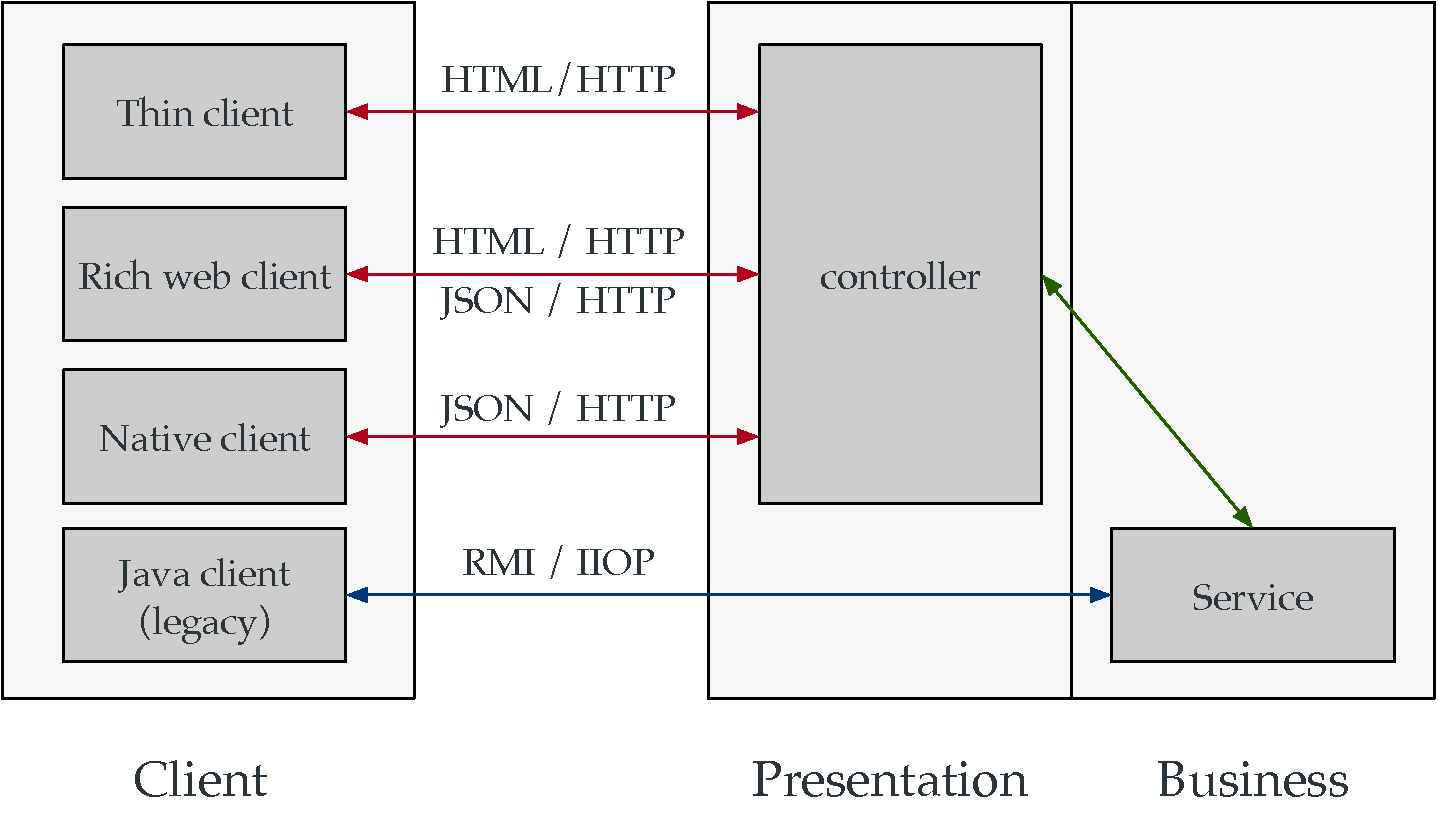
\includegraphics[width=1.0\linewidth]{Figures/client-tier.pdf}
	\caption{Interactions between the client and server tiers}
  \label{fig:client-tier}
\end{figure}

\section{Questions}

To answer these questions, you will need to have read the chapter but also to have done some research. Make sure that you are able to answer every question. Discuss your responses with your peers.

\begin{enumerate}
\item Let us consider Facebook. What kind of clients does the company use? Do not forget that a company always has external and internal applications.
\item What does the acronym AJAX mean and how does it relate to the client tier?
\item Give an example of a \ac{CLI} tool that you use and that is the client of a multi-tiered application.
\end{enumerate}


%************************************************
\chapter{The Presentation Tier}
\label{ch:presentation-tier}
%************************************************

\section{Introduction}

The presentation tier is located at the boundaries of the server side: it represents an entry point into the server. Its core responsibilities are to accept requests from clients, to figure out what business logic should be executed and finally to send responses in the appropriate format. 

The details of what happens in the presentation tier depends on type of client that sends the request: a thin client requesting web pages and a rich client requesting business data may involve different components on the server side. However, there are design patterns that apply in every situation. The objective of this chapter is to explore them. We will review the \ac{MVC}, the \ac{IoC} and the Pipes and Filters design patterns. After presenting them in generic terms, we will see how to concretely apply them with Java EE APIs and look at some code.

\section{The Model View Controller pattern}

\marginpar{MVC was first proposed in the context of GUI applications. In multi-tiered applications, MVC can mean different things. Rich clients and modern Javascript frameworks apply the traditional definition of the pattern. In the presentation tier, the pattern is applied quite differently. It is sometimes referred to as MVC2}

\ac{MVC} is one of the well-known design patterns and has been documented decades ago. It has its origin in the development of graphical user interfaces for desktop applications. The goal of the pattern is to clearly separate responsibilities between three software components. This leads to code that is easier to write, understand and maintain. In many software engineering courses and textbooks, the implementation of \ac{MVC} is illustrated with \ac{GUI} toolkits like Swing or Java FX. 

In the context of multi-tiered applications, be aware that \ac{MVC} can take different shapes and may be applied in different tiers. In the case of rich clients, \ac{MVC} takes its original form and is purely in the user interface domain. If you decide to use a client-side Javascript framework, such as Angular or React, you will be exposed to client-side \ac{MVC}. In the case of thin clients, \ac{MVC} is implemented on the server side, in the presentation tier. This changes quite a few things as the implementation does not involve a UI toolkit. In this chapter, we only consider the second situation. In other words, we describe a variation of the \ac{MVC} design pattern that operates on the server side. The key question is then to understand the relationship between the pattern components and the HTTP request-reply model.

\clearpage
\subsection{Description of the pattern}

The pattern involves the following participants:

\begin{itemize}
\item the \emph{model} is an object, or a graph of objects, that the user is interested in. Let's imagine that the user is accessing a product catalog: the model would be a List of Product objects, with properties such as Price and Description and with linked objects such as a List of Reviews or a Photo. Always keep in mind that you are manipulating graphs of objects: they need memory and bandwidth.
\item the \emph{view} is a component that produces a representation of the model. In the previous example, it could be a component that generates an HTML page with embedded images and hyperlinks. The view is generated on the server side, transferred to the client side, where it is finally rendered by a browser. In some cases, the representation is meant to be consumed by a human (e.g. HTML page or PNG image). In other cases, it is meant to be processed by a software agent (e.g. and XML or JSON payload).
\item the \emph{controller} is a component that reacts to user actions, is exposed to the details of the HTTP protocol and coordinates the work between the other components. In the case of thin web applications, whenever the user is taking an action (log in, access a product page, add a product in the shopping cart, send a message), he clicks on a link or a button, which causes the browser to send an HTTP request to the server. Every HTTP request is an event that represents a user action. It is comparable to a mouse event or a key event in a UI toolkit. When the server receives an HTTP request, it delegates its processing to the appropriate controller. The controller then has to extract information from the request (from the URL, the query string and/or the headers). The controller then decides how to generate a model and to ask a view to generate a representation of this model. Finally, the controller has to send the representation back to the client. At this stage, it is once again exposed to the details of the HTTP protocol.
\item the \emph{service} is a fourth component that is not strictly mandatory, but that is used very often to keep the code of the controllers small. In theory, a controller could create the model itself: by doing some sort of computation, by looking up information in a data store, etc. In practice, the controller will very often delegate this task to a service. In other words, it will handle the situation like this: ``Based on what I have seen in the URL and query string, I decide that Service A can handle the user action and generate a model for me. I also decide that View 1 can generate a representation of the model. I am going to coordinate the work between these two helpers.''
\end{itemize}

Figure \ref{fig:client-tier} shows the sequence of events for a typical user interaction round trip.
\begin{enumerate}
\item The user is visiting an online shop and is on a page that displays a list of products. For each product, there is a picture, a description, a price and an hyperlink entitled "Show details". The user has found an interesting product and clicks on the hyperlink. This where we start our exploration of the \ac{MVC} pattern.
\item The browser sends an HTTP request to the server. The method is \texttt{GET} and the URL is something like \url{http://shop.com/productsController?productId=4224&action=showDetails}. You can think of the HTTP request as an event, just like you would have a mouse event or a button even in a GUI toolkit.
\item On the server side, the HTTP request is routed to a component, which is the Controller in our pattern. Depending on the language and platform, the Controller might be an object or a function.
\item The Controller is lazy and tries to do as little as possible. Its first job is to figure out what other components can help him. Firstly, by looking at the attributes of the HTTP request (the URL, the query string, etc.), it will decide which business service can handle the request. It then calls the business service.
\item The Service does its job, which usually means getting some data, applying some business rules and computing a response. The response from the Service to the Controller is the Model in the pattern. It is usually an object or a graph of objects.
\item When the controller has received the Model, it looks for another helper: the View. Again, the controller is responsible to decide which of the available views can generate a representation of the Model. Usually, it looks at the HTTP headers sent by the client: the \texttt{Accept} header might indicate if the client prefers HTML or JSON. The Controller must have a way to pass the Model to the View, and to has the View to handle the last part of the processing. This depends on the platform and we will see the Java EE approach later in this chapter, with some code examples.
\item The last step is for the View to do the rendering and to prepare the response, which sent to the client.
\end{enumerate}

\begin{figure}[]
	\centering
    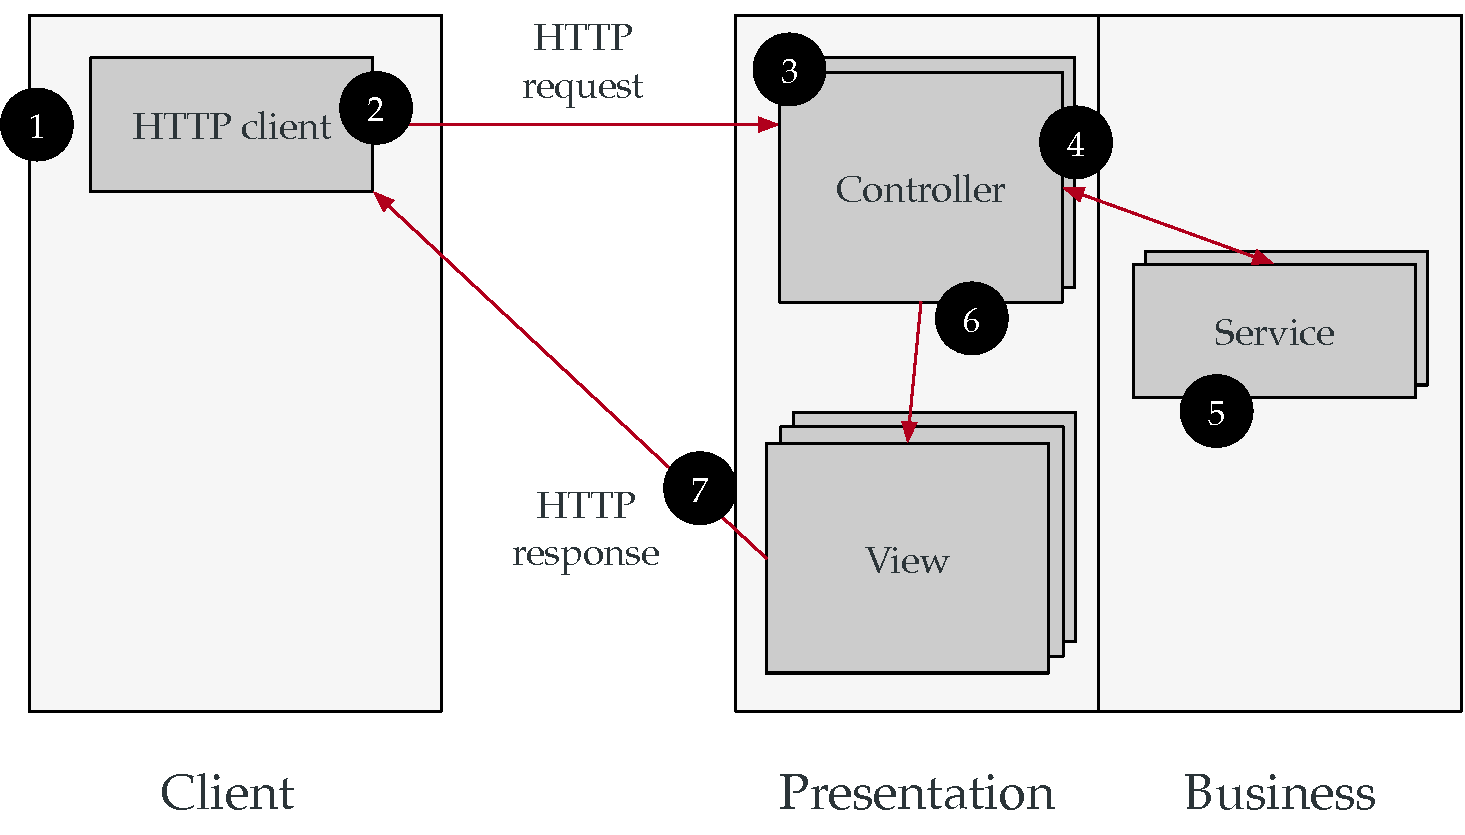
\includegraphics[width=1.0\linewidth]{Figures/MVC.pdf}
	\caption{The MVC design pattern in the presentation tier}
  \label{fig:mvc-in-presentation-tier}
\end{figure}

\subsection{Applying MVC in Java EE}

Let us know see how we can concretely implement the \ac{MVC} pattern with Java EE. For that purpose, we introduce two \ac{JSR}: the Servlet API and the \ac{JSP} API. 

A servlet is a Java object that implements a few methods, which are invoked when an HTTP request has been sent by a client. The responsibility of the servlet is to analyze the request (it has access to the URI, the HTTP headers, the body, etc.) and to prepare a response. A simple example is provided in Listing \ref{lst:quoteServlet}. 

\lstset{
	style=amt,
	language=Java,
	caption={A simple HTTP servlet},
	label={lst:quoteServlet},
}
\vspace{10pt}
\begin{minipage}{\linewidth}
\begin{lstlisting}[frame=single]
@WebServlet("/quote")
public class QuoteServlet extends HttpServlet {
  public void doGet(HttpServletRequest request, HttpServletResponse response) throws IOException {
    response.getWriter().println("<html>In cauda venenum.</html>");
  }
}
\end{lstlisting}
\end{minipage}

Let us review the code line by line:

\begin{itemize}
\item On line 1, the \texttt{@WebServlet} annotation is an instruction given to the application server. It is a way for the developer to state that when an incoming HTTP request targets the \texttt{/quote} URL, then the application server should forward it to this servlet. As we will see later, using this annotation is an alternative to the \texttt{web.xml} deployment descriptor.
\item On line 2, the developer creates a class by extending the \texttt{HttpServlet} abstract class, which is defined in the Servlet specification. The specification includes a Javadoc documentation for this class and its methods.
\item On line 3, the developer implements a method that will be invoked by the application server when the method in the incoming HTTP request is \emph{GET} (as opposed to \emph{POST}, \emph{PUT}, \emph{DELETE}, \emph{PATCH}, etc.).
\item The \texttt{doGet} method has two parameters. The \texttt{request} parameter is an object that represents a complete HTTP request. The \texttt{HttpServletRequest} class is also defined in the Servlet API specification. It provides getter methods to access the request method, URI, headers, etc. The \texttt{response} parameter represents the HTTP response. The developer uses this object to prepare the response sent to the client.
\item On line 4, the developer obtains a \texttt{PrintWriter} object and produces HTML markup that will be sent in the HTTP response body. The developer might also have added headers to the request. He might also have used an \texttt{OuputStream} object to send binary data to the client.
\end{itemize}

This is the simplest example to demonstrate how to build dynamic web applications in Java. But be aware that this example does not follow the \ac{MVC} pattern. The servlet is at the same time the Controller, the View and the Service (and for this reason, there is no real Model). Mixing HTML markup with Java code is a code smell. It is not rare to observe this in legacy applications and when it is the case, the maintenance is generally very painful.

\marginpar{Behind the scenes, the application server translates every \ac{JSP} template into Java source code, which it then compiles. The source code is actually a subclass of \texttt{HttpServlet}.}

Let us improve the code and introduce a View. For that purpose, we will use the \ac{JSP} technology. Historically, JSP was created a couple of years after the Servlet API. The technology provided a standard way to implement dynamic web pages and has been used extensively. It has evolved a lot over the years and many features have bean added either directly in its specification, or in companion \ac{JSR}s. Today, JSP is still supported by Java EE application servers and is a perfectly viable choice for building web applications. However, the technology has disappeared from official Java EE tutorials and seems to have lost traction with open source communities. Two factors can explain the situation:

\marginpar{\ac{JSP} has disappeared from the official Java EE tutorial. The last version that presents the technology and gives example is \href{https://docs.oracle.com/javaee/5/tutorial/doc/}{the Java EE 5 Tutorial.}}

\begin{itemize}
\item In 2004, the \ac{JSF} API was proposed as an alternative to JSP. The goal was to provide a solution for building component-based user interfaces, on the server side. This was a great idea, but it proved very hard to do. From our own experience, we can say that building web applications with \ac{JSF} was complex and time consuming. We moved away from the technology before it reached version 2.0, so things might have changed. Even if that is the case, we rarely see new projects adopt this technology, because the trend is now to build rich web clients. Hence, it is the surprising that the official Java EE guidelines put a very strong emphasis on \ac{JSF} and have even stopped presenting \ac{JSP}, a simpler and practical solution. Of course, if \ac{JSF} was widely adopted, it would be benefit certified Java EE application server vendors. The reason is that providing a \ac{JSF} implementation is mandatory for a fully compliant application server, but it is not for projects like Apache Tomcat.
\item At the same time, non-standard alternatives to \ac{JSP} have been provided by open source projects. \ac{JSP} is essentially a templating technology, and so are projects such as Thymeleaf, FreeMarker or Velocity. Frameworks that have been developed on top of Java EE, and in particular the very popular Spring MVC, do support \ac{JSP}, but often start by presenting other template engines.
\end{itemize}

Let us now how Java Server Pages look like and how they can be used in combination with servlets. The repository \href{https://github.com/SoftEng-HEIGVD/Teaching-HEIGVD-AMT-MVC-simple-example}{SoftEng-HEIGVD/Teaching-HEIGVD-AMT-MVC-simple-example}, hosted in GitHub, contains the code that we review here. Instructions for running the code with IntelliJ IDEA are provided in the repository \texttt{README.md} file.

\lstset{
	caption={Structure of the simple MVC project},
	label={lst:quotesProjectStructure}
}
\vspace{10pt}
\begin{minipage}{\linewidth}
\begin{lstlisting}[frame=single]
src/main
src/main/webapp
src/main/webapp/index.jsp
src/main/webapp/WEB-INF
src/main/webapp/WEB-INF/web.xml
src/main/webapp/WEB-INF/pages
src/main/webapp/WEB-INF/pages/view.jsp
src/main/java
src/main/java/ch
src/main/java/ch/heigvd
src/main/java/ch/heigvd/amt
src/main/java/ch/heigvd/amt/mvcsimple
src/main/java/ch/heigvd/amt/mvcsimple/business
src/main/java/ch/heigvd/amt/mvcsimple/business/QuoteGenerator.java
src/main/java/ch/heigvd/amt/mvcsimple/model
src/main/java/ch/heigvd/amt/mvcsimple/model/Quote.java
src/main/java/ch/heigvd/amt/mvcsimple/presentation
src/main/java/ch/heigvd/amt/mvcsimple/presentation/QuoteServlet.java
\end{lstlisting}
\end{minipage}

The structure of the project source files is shown in Listing \ref{lst:quotesProjectStructure}. Here is a description of the different packages and files:

\begin{itemize}
\item line 12: we use a namespace for the project: \texttt{ch.heivd.amt.mvcsimple}.
\item lines 17, 13, 6 and 15: we organize our classes based on the tiers of the architecture. We have controllers in the \texttt{presentation} package and services in the \texttt{business} package. We have views in the \texttt{pages} directory. The \texttt{model} package contains the classes that encapsulate business data and are used across tiers.
\item line 16: the Quote class is the \emph{model} in the application.
\item line 7: the view.jsp \ac{JSP} is the \emph{view} in the application.
\item line 18: the \texttt{QuoteServlet} class is the \emph{controller} in the application.
\item line 4: \texttt{WEB-INF} is a special directory and is present in every \texttt{.war} file.
\item line 5: \texttt{web.xml} is a \emph{deployment descriptor}. It describes the web application and is used by the application server at deployment time. In older versions of Java EE, the deployment descriptor was mandatory for all applications. Over time, the same information can be given to the application server via \emph{annotations} in the code. \emph{Warning}: the \texttt{web.xml} indicates the version of the Servlet API used by the application. Using an old version (e.g. by copying old examples found on the Web) may cause hard to debug problems.
\item line 6: the pages directory is located inside the \texttt{WEB-INF} directory. This is a security best practices. The Servlet specification states that it is not possible to access resources directly (i.e. it is not possible to type a URL in the browser to access them). The only way to reach them is to go via a controller. 
\end{itemize}

Now that we have seen the structure of the project, let us look at the code of the model (Listing\ref{lst:quotesProjectModel}), the controller (Listing\ref{lst:quotesProjectController}) and the view (Listing\ref{lst:quotesProjectView}).

\lstset{
	caption={The model class},
	label={lst:quotesProjectModel}
}
\vspace{10pt}
\begin{minipage}{\linewidth}
\begin{lstlisting}[frame=single]
package ch.heigvd.amt.mvcsimple.model;

public class Quote {

    private String author;
    private String citation;

    public Quote(String author, String citation) {
        this.author = author;
        this.citation = citation;
    }

    public String getAuthor() {
        return author;
    }

    public String getCitation() {
        return citation;
    }

}
\end{lstlisting}
\end{minipage}

Here are some comments about the \texttt{Quote} model class:

\begin{itemize}
\item lines 13 and 17: these two methods are often called getters, because they are used to get the value of an object property. The convention is to name these methods \texttt{getXXX()}, where \texttt{XXX} is the name of the property. Using this convention is not only a good practice that makes the code uniform and easy to read. It enables some of the magic that happens behind the scenes, because it facilitates dynamic code invocation. We will see a first simple example when we get to the code of the \ac{JSP} tempate. When we present the notion of \ac{ORM} later in the book, we will also explore the underlying mechanisms in more details. 
\item line 8: observe that the constructor allows us to define the state of the model object and that we did not implement any setter method. This is a good practice, when we want to work with immutable objects.
\end{itemize}

\lstset{
	caption={The controller class},
	label={lst:quotesProjectController}
}
\vspace{10pt}
\begin{minipage}{\linewidth}
\begin{lstlisting}[frame=single]
package ch.heigvd.amt.mvcsimple.presentation;

import ch.heigvd.amt.mvcsimple.business.QuoteGenerator;
import ch.heigvd.amt.mvcsimple.model.Quote;

import javax.servlet.ServletConfig;
import javax.servlet.ServletException;
import java.io.IOException;
import java.util.List;

public class QuoteServlet extends javax.servlet.http.HttpServlet {

    private QuoteGenerator service; // we will see later how to replace this with dependency injection

    @Override
    public void init(ServletConfig config) throws ServletException {
        super.init(config);
        service = new QuoteGenerator();
    }

    protected void doGet(javax.servlet.http.HttpServletRequest request, javax.servlet.http.HttpServletResponse response) throws javax.servlet.ServletException, IOException {
        List<Quote> model = service.generateQuotes();
        request.setAttribute("quotes", model);
        request.getRequestDispatcher("/WEB-INF/pages/view.jsp").forward(request, response);
    }
}
\end{lstlisting}
\end{minipage}

Here are some comments about the \texttt{QuoteServlet} controller class:

\begin{itemize}
\item line 11: we implement a servlet, which extends the abstract \texttt{HttpServlet} class.
\item line 13: we use service, which we instantiate ourselves for the moment, when the servlet is created by the application server (line 18)
\item line 21: we implement the \texttt{doGet} method, which receives a request and a response in parameter. In the method, we invoke the service and obtain a model (a list of quotes). With \texttt{request.setAttribute}, we attach the model to the request. This will allow other components, and in particular the \ac{JSP} template, to retrieve the model down the processing chain.
\item line 24: the way to pass the request to the view is to obtain a request dispatcher for the target template and to call the forward method.
\end{itemize}

\lstset{
	caption={The view template},
	language=html,
	label={lst:quotesProjectView}
}
\vspace{10pt}
\begin{minipage}{\linewidth}
\begin{lstlisting}[frame=single]
<%@ page contentType="text/html;charset=UTF-8" language="java" %>
<%@ taglib prefix="c" uri="http://java.sun.com/jsp/jstl/core" %>
<html>
  <head>
    <title>Quotes</title>
  </head>
  <body>
    <h2>Quotes</h2>
    <ul>
      <c:forEach items="${quotes}" var="quote">
        <li>${quote.author} : "${quote.citation}"</li>
      </c:forEach>
    </ul>
  </body>
</html>
\end{lstlisting}
\end{minipage}

Here are some comments about the \texttt{page.jsp} view template:

\begin{itemize}
\item line 2: in this example, we use the \ac{JSTL} tag library. Tag libraries are a mechanism for defining custom tags, which can be used in page templates. Here, we specify that \ac{JSTL} tags will be prefixed by \texttt{c:} (line 10). Warning: a fully compliant Java EE application server has to provide an implementation of \ac{JSTL}. Tomcat, however, is not fully compliant. Therefore, if you deploy the application in Tomcat, you will need to bundle the \ac{JSTL} \texttt{.jar} file. When using maven, the \texttt{scope} of a dependency defines whether the dependency is bundled in the \texttt{.war} file or if it is \texttt{provided} by the application server runtime environment. 
\item line 10: the \texttt{c:forEach} tag allows us to iterate over a collection. In this case, \texttt{\$\{quotes\}} means that the engine will try to find a model named \texttt{quote} in different scopes (page, request, session, application). Remember that in the servlet, we used the method \texttt{setAttribute('quotes', model)}, which is why the template can retrieve the model.
\item line 11: in the loop, the \texttt{quote} variable represents one quote in the list. With the expressions \texttt{\$\{quote.author\}} and \texttt{\$\{quote.citation\}}, we can retrieve the properties defined in the model class \texttt{Quote}). How does that work? Remember that we talked about naming conventions and getter methods. Behind the scenes, when the template engine sees \texttt{quote.citation}, it computes the name of a method (\texttt{get} + capitalized name of the property) and attempts to make a dynamic call to this method. The Java mechanism that makes this possible is the Java Reflection API.
\end{itemize}

\lstset{
	caption={The deployment descriptor},
	language=xml,
	label={lst:quotesProjectDeploymentDescriptor}
}
\vspace{10pt}
\begin{minipage}{\linewidth}
\begin{lstlisting}[frame=single]
<web-app xmlns="http://xmlns.jcp.org/xml/ns/javaee"
         xmlns:xsi="http://www.w3.org/2001/XMLSchema-instance"
         xsi:schemaLocation="http://xmlns.jcp.org/xml/ns/javaee
		 http://xmlns.jcp.org/xml/ns/javaee/web-app_3_1.xsd"
         version="3.1">
  <display-name>Archetype Created Web Application</display-name>
  <servlet>
    <servlet-name>QuoteServlet</servlet-name>
    <servlet-class>ch.heigvd.amt.mvcsimple.presentation.QuoteServlet</servlet-class>
  </servlet>
  <servlet-mapping>
    <servlet-name>QuoteServlet</servlet-name>
    <url-pattern>/quotes</url-pattern>
  </servlet-mapping>
</web-app>
\end{lstlisting}
\end{minipage}

Here are some comments about the \texttt{web.xml} deployment descriptor:

\begin{itemize}
\item line 1-5: this tag specifies the version of the Servlet API used by the application. Warning: be careful when using old examples found on the Web, because specifying an old version here will mean that some mechanisms introduced later will not work (for instance, the expression language used in \ac{JSP} templates).
\item lines 7-10: we define a servlet, by giving it a name and a fully qualified class name.
\item lines 11-14: we define a mapping between a URL and a servlet. This is a way to tell the application server: whenever an HTTP request comes in and matches the pattern, then invoke this servlet.
\item note that the deployment descriptor is now optional and can be replaced by annotations in the code. You will still encounter this file in older projects (and some teams prefer to declare all attributes in a central location, instead of having the scattered in different source files). 
\end{itemize}

\section{The Inversion of Control design pattern}

The \ac{IoC} principle is pervasive in client-side and server-side frameworks. In the context of Java EE, it is applied in several tiers. We will see concrete code examples later, but let us start with a presentation of the concept.

\subsection{Description of the pattern}

\marginpar{When using a library, the developer controls the flow. He decides when to call functions provided by the library.}

What does it mean to \emph{inverse} the \emph{control}? Control refers to the control of the flow in a program. In simple programs, the developer controls the flow. He writes functions, which may delegate work to other functions, in a top-down fashion. A \emph{library} is a collection of functions that can be shared and reused across programs. The developer using a library decides when to call the provided functions. For instance, when implementing a password management function, the developer might call a function provided by an encryption library.

\marginpar{When using a framework, the developer does not control the flow anymore. He provides code that is called by the framework, when needed.}

Inverting the flow of control means that the developer does not call a function, but rather provides a function that \emph{will called when it makes sense}. This approach is at the core of object-oriented \emph{frameworks}. A framework implements a generic behaviour with a set of abstract classes that collaborate with each other. The developer creates an application by extending the framework classes and implementing concrete methods. But the developer does not control the flow, the framework does. At some point, the framework decides that it is time to create an instance of the concrete class provided by the developer, or to invoke one of its method.

To illustrate this mechanism, think about a graphical editor, allowing the user to create shapes on a canvas and to apply various styles. The application provides a user interface, with menus, windows, palettes, etc. It also implements data management, printing, etc. All these behaviours are implemented by classes, which collaborate with each other. If the graphical editor is implemented as an object-oriented framework, then the developer might be able to augment its behaviour by extending a \texttt{Shape} class. In this class, he might implement methods like \texttt{draw}, \texttt{load}, \texttt{save}, \texttt{getStyleProperties}, \texttt{applyStyleProperties}, etc. The developer provides implementations and understands that it is the framework that will invoke them when needed.

The difference between a library and a framework is shown in Figure \ref{fig:library-vs-framework}. The pseudo-code indicates that a program \emph{calls} a library, but \emph{is called} by a framework. This is sometimes described as the \emph{Hollywood Principle}.

\begin{figure}[]
	\centering
    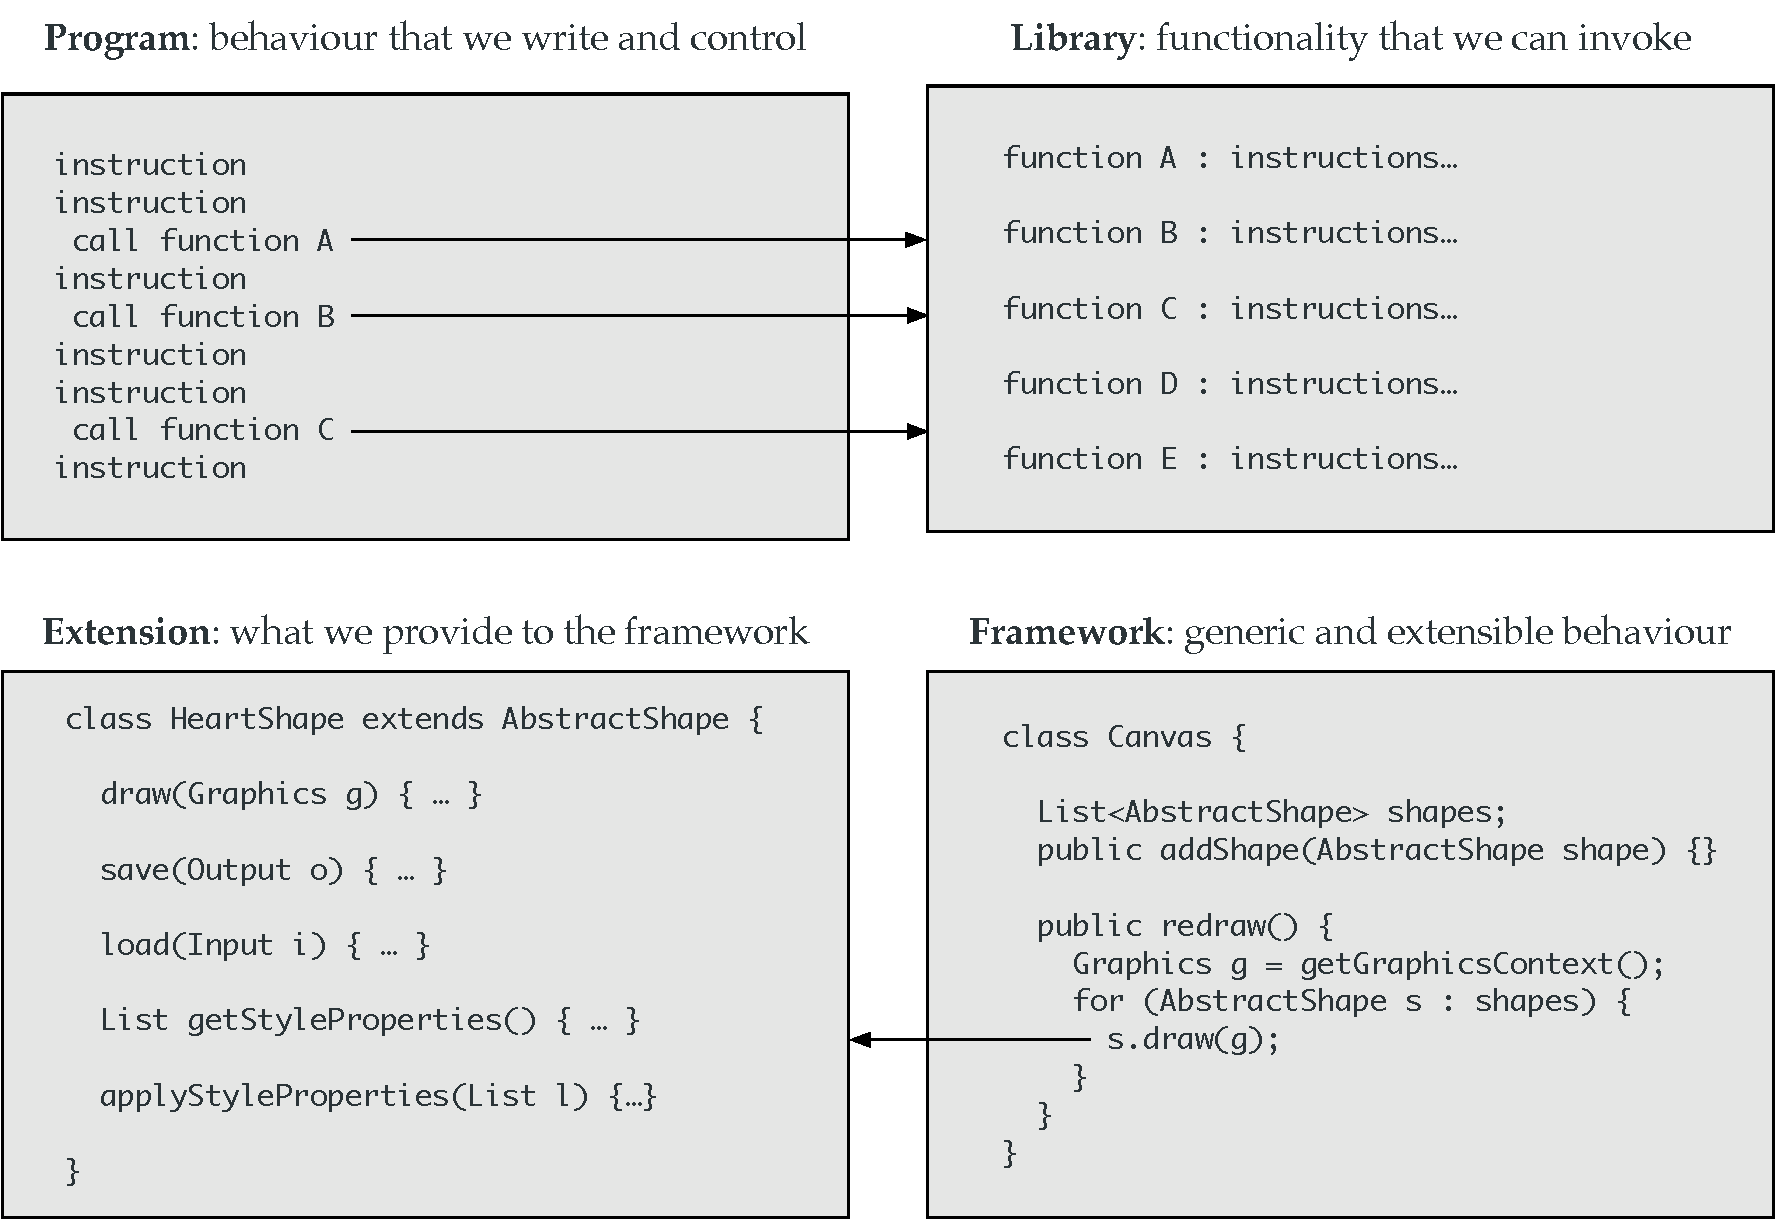
\includegraphics[width=1.0\linewidth]{Figures/frameworkVsLibrary.pdf}
	\caption{Inversion of Control: libraries vs frameworks}
  \label{fig:library-vs-framework}
\end{figure}

\subsection{IoC in the Java EE presentation tier}

As a matter of fact, we have already seen how the \ac{IoC} pattern is applied in the presentation tier, when using servlets.

Let us consider how a developer could build a dynamic web application in Java, but without a Java EE application server. In this case, the developer would use classes from the \texttt{java.net} and \texttt{java.io} packages. He would create a server socket and accept connection requests in a loop. For every new client, he would read the incoming HTTP request line by line. He would prepare a response and send it back to the client, via the socket. Clearly, the developer would control the flow and make calls to classes and methods provided by the Java runtime environment.

The code that we have seen in this chapter follows a different logic. We use the application server as a framework. It implements the generic behavior of any web application: it manages the server socket and accepts client requests. Of course, without us, it is an empty shell and is not able to send meaningful responses to the clients. When we have written the servlet class, we have used an extension point provided by the framework. We have implemented a method that can be called by the application server \emph{at the right time}. But when does the application server decides what is \emph{the right time}? This is where the annotation in Listing \ref{lst:quoteServlet} or the servlet mapping in Listing \ref{lst:quotesProjectDeploymentDescriptor} comes in. The developer uses these mechanisms to register his extension and to specify that it should be called when an incoming HTTP request has certain attributes. The URL is first used to identify the servlet class, the HTTP method is then used to identify the method within this class.

\section{The Pipes and Filters pattern}

The Pipes and Filters pattern can be applied when the processing of a task can be decomposed in a number of steps, and when the steps can be handled by independent, reusable building blocks. The pattern is not specific to multi-tiered applications and can be applied in a wide range of situations. One example is the usage of the \emph{pipe} operator to combine unix commands in a sequence. Another example is the use of the \texttt{Filter} classes in the \texttt{java.io} package, which make it possible to apply different transformations when reading and writing data streams.

\subsection{Description of the pattern}

The pattern is represented in Figure \ref{fig:pipesAndFilters}. The \emph{source} produces a \emph{stream} of \emph{tasks}, which enter a processing \emph{pipeline}. The \emph{pipeline} is not a monolithic piece of code. Instead, it is created by assembling a series of \emph{filters}. Every \emph{filter} performs a well-defined function on the \emph{task}. This means that the \emph{task} can be modified or augmented before being passed to the next \emph{filter}. At the end, the sink receives the result of the computation. The great thing about this pattern is that it is possible to reuse \emph{filters} in different types of \emph{pipelines}. 

\begin{figure}[]
	\centering
    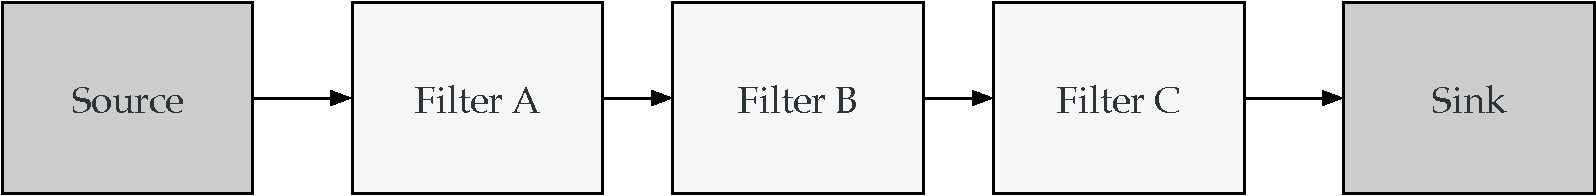
\includegraphics[width=1.0\linewidth]{Figures/pipesAndFilters.pdf}
	\caption{The Pipes and Filters design pattern}
  \label{fig:pipesAndFilters}
\end{figure}

\begin{figure}[]
	\centering
    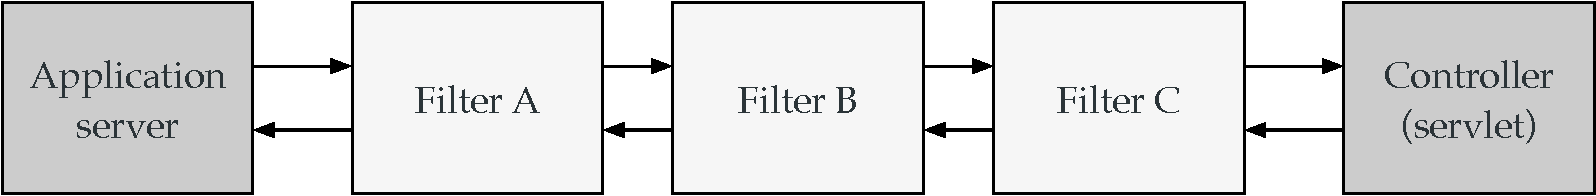
\includegraphics[width=1.0\linewidth]{Figures/pipesAndFiltersHttp.pdf}
	\caption{The Pipes and Filters design pattern in the presentation tier}
  \label{fig:pipesAndFiltersHttp}
\end{figure}

\subsection{Pipes and Filters in the presentation tier}

When applying the pattern in the presentation tier, the tasks processed by the pipeline are the HTTP requests. The application server, which receives the request, is the source. HTTP requests are processed by several filters before they reach the controller. In fact, as shown in Figure \ref{fig:pipesAndFiltersHttp}, the pattern is applied twice: HTTP responses produced by the controller also go through the sequence of filters, which have the opportunity to modify them.

But what is the reason for using filters and what kind of processing is typically done in these components? These are common use cases:

\begin{itemize}
\item \emph{auditing}: a filter can just observe the requests and generate an audit log
\item \emph{authorization}: a filter can decide if the user making the request has the right to do it
\item \emph{compression}: a filter can decompress incoming requests and compress outgoing responses
\item \emph{encryption}: a filter can decrypt requests and encrypt responses
\item \emph{caching}: a filter can optimize performance by reusing previously generated responses (in this case, the filter may short-circuit the pipeline)
\end{itemize}

In order to create custom servlet filters, the developer needs to implement the \texttt{Filter} interface, which defines three methods: \texttt{init(FilterConfig filterConfig)}, \texttt{destroy()} and most importantly \texttt{doFilter(ServletRequest request, ServletResponse response, FilterChain chain)}. An example is shown in Listing \ref{lst:servletFilterExample}. Here are some explanations about the code:

\begin{itemize}
\item line 7: the annotation registers the filter, so that \ac{IoC} can happen
\item line 8: we implement the \texttt{Filter} interface
\item line 12: \texttt{doFilter} is called when the requests advances in the pipeline. Other filters might have been called before, other filters might be called after. The \texttt{chain} parameter represents the processing pipeline.
\item line 19: to test the pipeline, we simply attach a String model to the request. This model will be available in other filters, in the controller servlet and in the \ac{JSP} template.
\item line 21: we pass the request further down the chain.
\item line 23: when the call returns, we have the ability to inspect the response and to modify it. However, if we want to do that, we need to wrap \texttt{resp} in a special object, to capture the output stream in memory.
\end{itemize}

\lstset{
	caption={A servlet filter example},
	language=java,
	label={lst:servletFilterExample}
}
\vspace{10pt}
\begin{minipage}{\linewidth}
\begin{lstlisting}[frame=single]
package ch.heigvd.amt.mvcsimple.presentation;

import javax.servlet.*;
import javax.servlet.annotation.WebFilter;
import java.io.IOException;

@WebFilter(filterName = "CustomFilter", urlPatterns = "/*")
public class CustomFilter implements Filter {
    public void destroy() {
    }

    public void doFilter(ServletRequest req, ServletResponse resp, FilterChain chain) throws ServletException, IOException {
        /*
         The pipeline is first going from the app server towards the controller.
         We can log the request, transform the request. We can also block the 
         request (by not calling chain.doFilter(req, resp);
         */

        req.setAttribute("computedByFilter", "yellow");

        chain.doFilter(req, resp);

        /*
         We are on the way back. Now, we can transform the response. But to
         do that, we would need to send a wrapper to the chain in the previous 
         call. You can find an example in the Java EE 5 tutorial
         */
    }

    public void init(FilterConfig config) throws ServletException {
    }

}
\end{lstlisting}
\end{minipage}

\section{Questions}

To answer these questions, you will need to have read the chapter but also to have done some research. Make sure that you are able to answer every question. Discuss your responses with your peers.

\begin{enumerate}
\item \emph{How does one implement HTML form processing in Java EE?} Consider the scenario where the user arrives on a page, fills out three fields (\texttt{first name}, \texttt{last name} and \texttt{e-mail address}) and presses a \texttt{Register} button. We want to process the event on the server side and to validate the data entered by the user (the fields cannot be empty and the e-mail address must contain an @ sign). What code do you have to write?
\item \emph{What is the difference between the request, session and application scopes in the servlet API?} The method \texttt{setAttribute} is available in the \texttt{HttpServletRequest}, \texttt{HttpSession} and \texttt{ServletContext} classes. What is the difference and when should they be used?
\item \emph{Why do we have to be careful with the \texttt{HttpSession} object?}. The Servlet API makes it very easy to store objects in the session. While it is practical to use this feature to build stateful applications on top of the stateless HTTP protocol, it does not come for free. There are at least risks or drawbacks to be aware of. What are they?
\item \emph{How do we deal with relative links in \ac{JSP} templates?}. It is possible to deploy several applications in the same applications server. For this to work, every application is assigned a \emph{context root}. In order to generate links to CSS files and other assets, it is often necessary to include the context root in the path and it is a bad idea to hard-code the value in the template. What is the solution to this problem?
\end{enumerate}



%
%\chapter{Business tier}\label{ch:first-steps}
%\section{The Dependency Injection pattern}
%\section{Enterprise Java Beans}
%
%\chapter{Integration tier}\label{ch:first-steps}
%\section{The Data Access Object pattern}
%\section{Java DataBase Connectivity}
%\section{Boiler plate code and reflection}
%\section{Object Relational Mapping}
%

\ctparttext{This part presents a selection of frameworks that have been built on top of \ac{Java EE} APIs and are currently very popular in the market. These frameworks aim to make developers more productive, by providing additional capabilities and by hiding some of the implementation details. They also address the evolution towards the cloud and micro-services architecture. This topic has been a gap in the Java EE specification (this will be one focus area for its future versions) for a long time, which is one reason to explain the popularity of the frameworks.
}

\part{Modern Java EE}\label{pt:old-style}
%
%\chapter{Micro-services with Springboot}\label{ch:first-steps}
%\section{The Spring Framework}
%\section{The Springboot Project}
%\section{Micro-services}
%
%\chapter{Persistence with Spring Data}\label{ch:first-steps}
%
%\chapter{APIs with Spring Data REST}\label{ch:first-steps}
%

\ctparttext{This part presents software engineering practices that are recommended when developing multi-tiered applications. The goal of these practices is to improve the productivity of the team and the quality of the developed product. A lot of these practices are related to testing, which is a broad subject. Both functional and non-functional requirements need to be tested. Different techniques and tools can be used for this purpose. Some of them are presented in the following chapters, with concrete case studies and examples.}

\part{Software engineering practices}\label{pt:old-style}
%************************************************
\chapter{Performance and Load Testing}
\label{ch:performance-load-testing}
%************************************************

\section{Introduction}

When creating a software product, the team has two consider two types of requirements:

\begin{itemize}
\item the \emph{functional requirements} specify \emph{what} the software should do. When doing a use case analysis, the team identifies the actors (the categories of users and external systems) which interact with the system. The team also enlists the features provided by the system as a list of use cases and scenarios.
\item The \emph{non-functional requirements} specify and quantify various qualities that the system should have. For instance, the team should assess what are the needs in terms of performance, scalability, availability, security, maintainability, manageability, etc. This is a critical part of the analysis, because it should drive the architecture of the system. Making a sound architectural decision is about making the right \emph{tradeoff} between the cost of a solution and its impact on non-functional requirements. For instance, availability is always somewhat important. It is possible, but very complex and costly to build systems with a 99.999\% uptime. The first task is to define what is the appropriate availability level for the system. The second task is to propose a technical design that is expected to reach that level. The third, very important and often overlooked, is to actually measure if the target level can be reached.
\end{itemize}

In this chapter we take a look at the performance of the application, one of the non-functional requirements. We show how it is possible to measure the performance of a web application, also when it is is under heavy load. We present Apache JMeter, an open source tool that supports this testing activity.

\section{Testing web applications with Apache JMeter}

\subsection{Installation and configuration}
\subsection{Concepts}
\subsection{Scenarios and virtual users}

\section{Case study: thread-safety of the Servlet API}

\section{Case study: impact of caching in multi-tiered applications}

\section{Questions}

To answer these questions, you will need to have read the chapter but also to have done some research. Make sure that you are able to answer every question. Discuss your responses with your peers.




%
%\chapter{Load and performance testing}\label{ch:first-steps}
%\chapter{Contract-first development of REST APIs}\label{ch:first-steps}
%\chapter{Continuous integration}\label{ch:first-steps}
%\chapter{User Interface testing}\label{ch:first-steps}
%\chapter{Behaviour Driven Design}\label{ch:first-steps}


%\include{multiToC} % <--- just debug stuff, ignore for your documents
% ********************************************************************
% Backmatter
%*******************************************************
%\appendix
%\renewcommand{\thechapter}{\alph{chapter}}
%\cleardoublepage
%\part{Appendix}
%\include{Chapters/Chapter0A}
%********************************************************************
% Other Stuff in the Back
%*******************************************************
%\cleardoublepage\include{FrontBackmatter/Bibliography}
%\cleardoublepage\include{FrontBackmatter/Declaration}
%\cleardoublepage\include{FrontBackmatter/Colophon}
% ********************************************************************
% Game Over: Restore, Restart, or Quit?
%*******************************************************
\end{document}
% ********************************************************************
